\section{测序技术}

\subsection{测序技术的发展}
\begin{frame}
  \frametitle{测序 | 简介}
  \begin{block}{DNA测序}
DNA测序(DNA sequencing)是指分析特定DNA片段的碱基序列,也就是腺嘌呤(A)、胸腺嘧啶(T)、胞嘧啶(C)与鸟嘌呤(G)的排列方式。
  \end{block}
  \pause
  \begin{block}{RNA测序}
RNA测序则通常将RNA提取后,反转录为DNA后使用DNA测序的方法进行测序。
  \end{block}
\end{frame}

\begin{frame}
  \frametitle{测序 | 历史}
  \begin{figure}
    \centering
    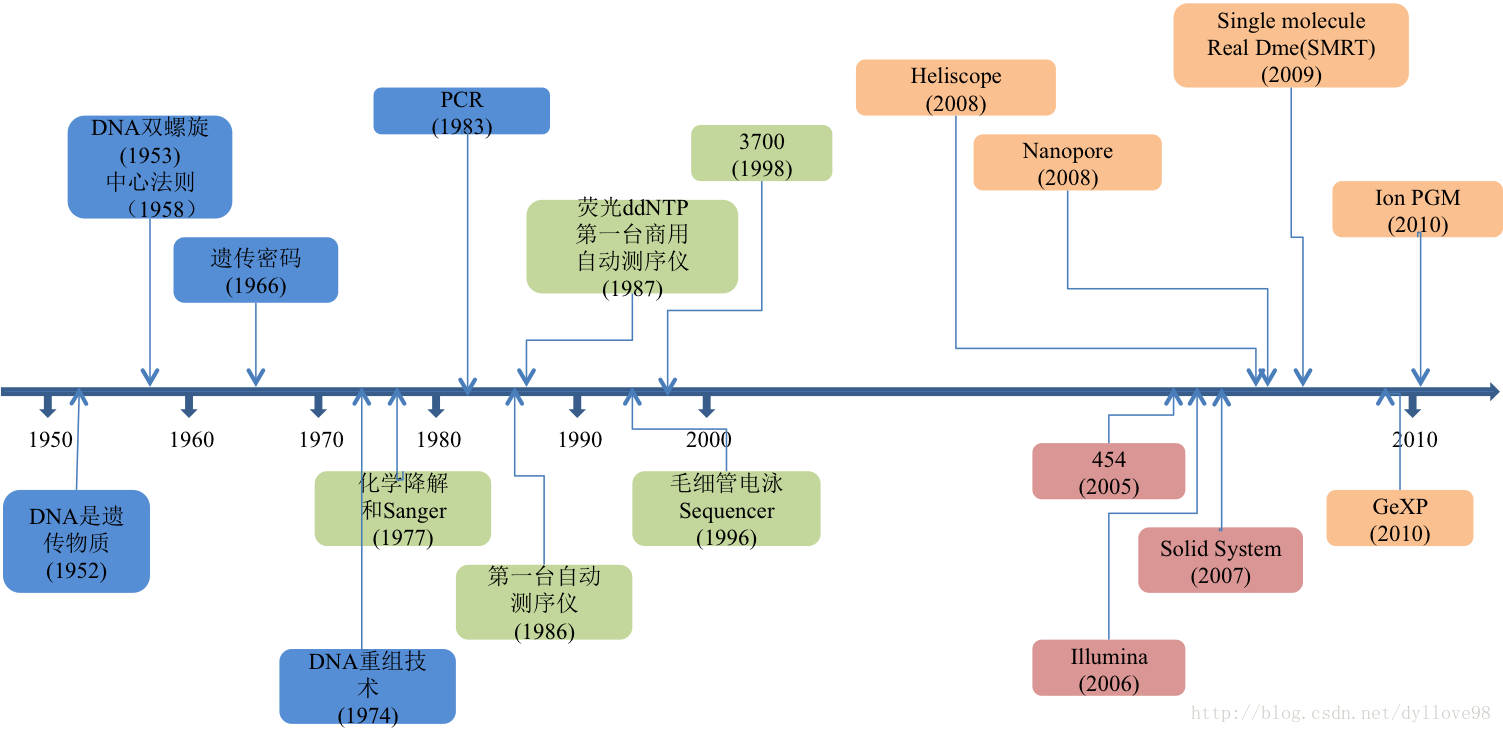
\includegraphics[width=0.9\textwidth]{c2_genomics/sequencing_timeline_01.png}
  \end{figure}
\end{frame}

\begin{frame}
  \frametitle{测序 | 历史}
  \begin{figure}
    \centering
    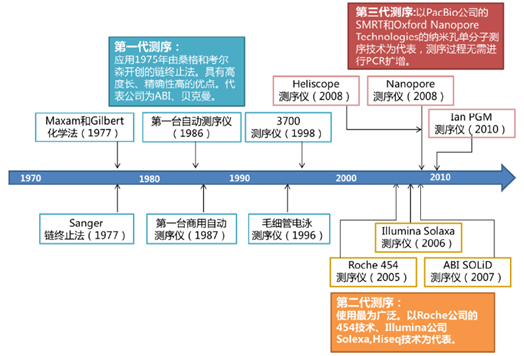
\includegraphics[width=0.9\textwidth]{c2_genomics/sequencing_timeline_02.png}
  \end{figure}
\end{frame}

\subsection{第一代测序技术}
\begin{frame}
  \frametitle{测序 | 第一代 | 简介}
   \begin{itemize}
     \item 1975年,弗雷德里克·桑格(Frederick Sanger)和艾伦·库尔森(Alan Coulson),“加减测序法技术”;改进后为链终止法(chain termination method),即桑格测序法
     \item 1977年,哈佛大学的沃尔特·吉尔伯特(Walter Gilbert)和艾伦·马克萨姆(Allan Maxam),链降解,马克萨姆-吉尔伯特测序(Maxam-Gilbert法,又称化学测序法)
   \end{itemize}
\end{frame}

\begin{frame}
  \frametitle{测序 | 第一代 | 化学测序法}
  \begin{block}{化学测序法}
马克萨姆-吉尔伯特测序(Maxam-Gilbert sequencing)是一项由阿伦·马克萨姆与沃尔特·吉尔伯特于1976~1977年间开发的DNA测序方法。此项方法基于:对核碱基特异性地进行局部化学变性,接下来在变性核苷酸毗邻的位点处DNA骨架发生断裂。\\
\vspace{1em}
最初的桑格法须要在每次测序之前克隆得到单链DNA产物,因此马克萨姆-吉尔伯特测序法发表后迅速得到了推广,因为被纯化的DNA可被直接使用。然而,随着链终止法的改良,马克萨姆-吉尔伯特测序逐渐失宠,这是由于:技术复杂性阻碍其成为标准分子生物学套装使用、大量使用危险药品以及难于扩大规模。
  \end{block}
\end{frame}

\begin{frame}
  \frametitle{测序 | 第一代 | 化学测序法}
  \begin{figure}
    \centering
    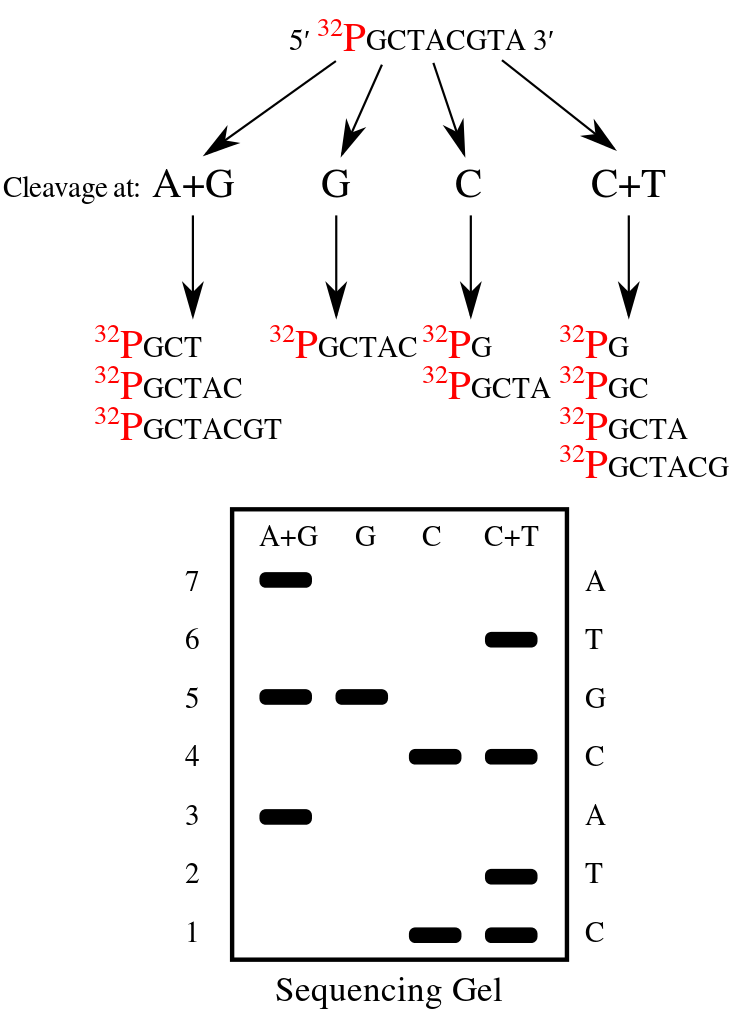
\includegraphics[width=0.48\textwidth]{c2_genomics/sequencing_mg_01.png}
  \end{figure}
\end{frame}

\begin{frame}
  \frametitle{测序 | 第一代 | 桑格测序法}
  \begin{block}{桑格测序法}
Sanger(桑格)双脱氧链终止法是弗雷德里克·桑格(Frederick Sanger)于1975年发明的。测序过程需要先做一个聚合酶连锁反应(PCR)。PCR过程中,双脱氧核糖核苷酸可能随机的被加入到正在合成中的DNA片段里。由于双脱氧核糖核苷酸少了一个氧原子,一旦它被加入到DNA链上,这个DNA链就不能继续增加长度。最终的结果是获得所有可能获得的、不同长度的DNA片段。\\
\vspace{1em}
目前最普遍最先进的方法,是将双脱氧核糖核苷酸进行不同荧光标记。将PCR反应获得的总DNA通过毛细管电泳分离,跑到最末端的DNA就可以在激光的作用下发出荧光。由于ddATP, ddGTP, ddCTP, ddTTP(4种双脱氧核糖核苷酸)荧光标记不同,计算机可以自动根据颜色判断该位置上碱基究竟是A,T,G,C中的哪一个。
  \end{block}
\end{frame}

\begin{frame}
  \frametitle{基因组学 | 测序 | 第一代 | 桑格测序法}
  \begin{block}{原理}
双脱氧链终止法采用DNA复制原理。Sanger测序反应体系中包括目标DNA片断、脱氧三磷酸核苷酸(dNTP)、双脱氧三磷酸核苷酸(ddNTP)、测序引物及DNA聚合酶等。\\
\vspace{1em}
测序反应的核心就是其使用的ddNTP:由于缺少3'-OH基团,不具有与另一个dNTP连接形成磷酸二酯键的能力,这些ddNTP可用来中止DNA链的延伸。此外,这些ddNTP上连接有放射性同位素或荧光标记基团,因此可以被自动化的仪器或凝胶成像系统所检测到。
  \end{block}
\end{frame}

\begin{frame}
  \frametitle{测序 | 第一代 | 桑格测序法}
  \begin{block}{概述}
    每个反应含有所有四种脱氧三磷酸核苷酸(dNTP)使之扩增,并混入限量的一种不同的双脱氧三磷酸核苷酸(ddNTP)使之终止。由于ddNTP缺乏延伸所需要的3'-OH基团,使延长的寡聚核苷酸选择性地在G、A、T或C处终止,终止点由反应中相应的ddNTP而定。\\
\vspace{1em}
每一种dNTPs和ddNTPs的相对浓度可以调整,使反应得到一组长几个至千以上个、相差一个碱基的一系列片断。它们具有共同的起始点,但终止在不同的核苷酸上,可通过高分辨率变性凝胶电泳分离大小不同的片段,凝胶处理后可用X-光胶片放射自显影或非同位素标记进行检测。
  \end{block}
\end{frame}

\begin{frame}
  \frametitle{测序 | 第一代 | 桑格测序法}
  \begin{block}{优势}
    \begin{itemize}
      \item 最长可测定600-1000bp的DNA片断
      \item 对重复序列和多聚序列的处理较好
      \item 序列准确性高,高达99.999\%
      \item 测序的“黄金标准”
    \end{itemize}
  \end{block}
  \pause
  \begin{block}{缺点}
    \begin{itemize}
      \item 通量较低(在24h内可测定的DNA分子数一般不超过10,000个)
      \item 每碱基测序成本较高
      \item 不适合大规模平行测序
    \end{itemize}
  \end{block}
\end{frame}

\begin{frame}
  \frametitle{测序 | 第一代 | 桑格测序法}
  \begin{figure}
    \centering
    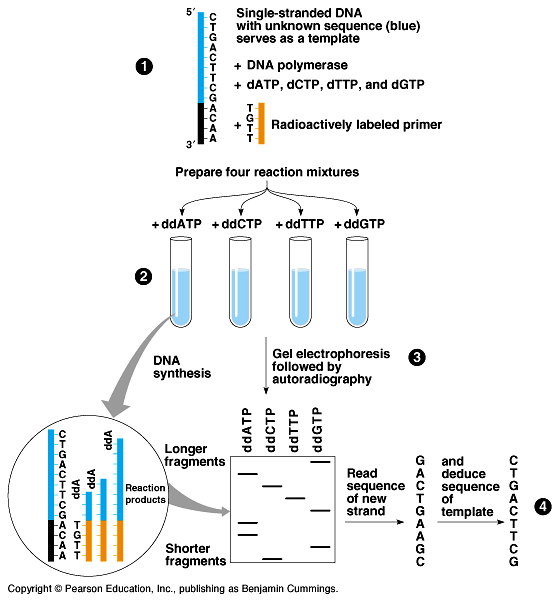
\includegraphics[width=0.6\textwidth]{c2_genomics/sequencing_sanger_01.png}
  \end{figure}
\end{frame}

\begin{frame}
  \frametitle{测序 | 第一代 | 桑格测序法}
  \begin{figure}
    \centering
    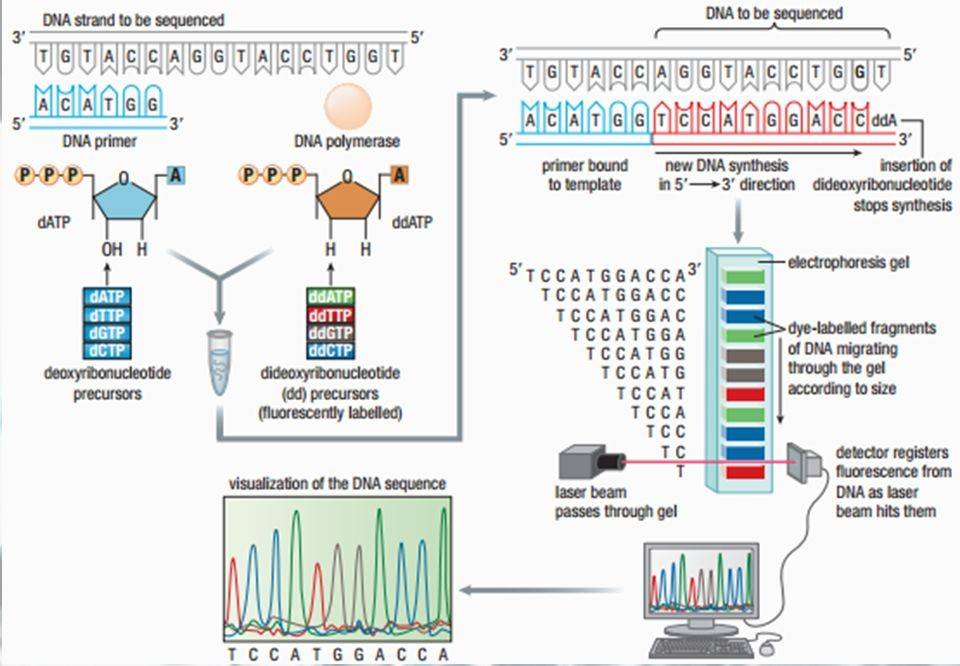
\includegraphics[width=0.9\textwidth]{c2_genomics/sequencing_sanger_04.jpg}
  \end{figure}
\end{frame}

\subsection{第二代测序技术}
\begin{frame}
  \frametitle{测序 | 第二代 | 引言}
  \begin{block}{Reads}
    \begin{columns}
      \column{0.2\textwidth}
      \column{0.3\textwidth}
一个完美的人 \\ ,不是寻找一 \\ 眼光,欣赏那 \\ 爱,不是寻找 \\ 是学会用完美 \\  不完美的人。 \\
      \column{0.3\textwidth}
是寻找一个完 \\ 的人,而是学 \\ 完美的眼光, \\ ,欣赏那个并 \\ 完美的人,而 \\ 那个并不完美  \\
      \column{0.2\textwidth}
    \end{columns}
  \end{block}
  \pause
  \pause
  \pause
  \pause
  \begin{block}{基因组}
    爱,不是寻找一个完美的人,而是学会用完美的眼光,欣赏那个并不完美的人。——《哈尔的移动城堡》
  \end{block}
\end{frame}

\begin{frame}
  \frametitle{测序 | 第二代 | 引言}
  \begin{block}{Reads}
    \begin{columns}
      \column{0.2\textwidth}
      \column{0.3\textwidth}
      who you are \\ are, but \\ I love you \\ not for who \\ am with you \\ who I am \\
      \column{0.3\textwidth}
      love you not \\ but for who \\ you not for \\ for who I \\ with you. \\ you are, \\
      \column{0.2\textwidth}
    \end{columns}
  \end{block}
  \pause
  \pause
  \pause
  \pause
  \begin{block}{基因组}
    I love you not for who you are, but for who I am with you. ——《剪刀手爱德华》
  \end{block}
\end{frame}

\begin{frame}
  \frametitle{测序 | 第二代 | 引言}
  \begin{figure}
    \centering
    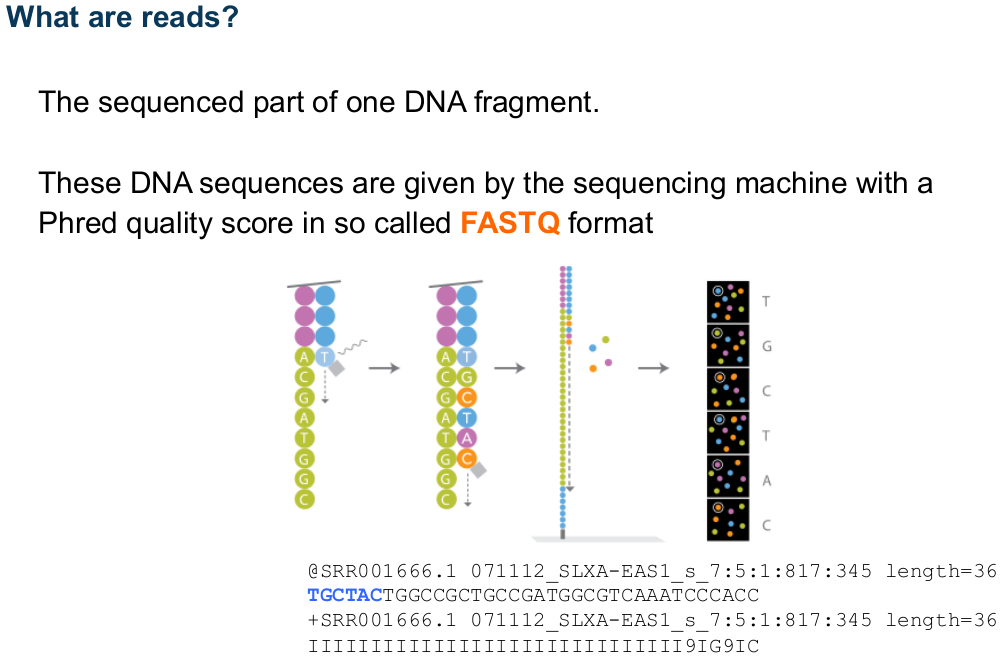
\includegraphics[width=\textwidth]{c2_genomics/ngs_reads_seq_02.png}
  \end{figure}
\end{frame}

\begin{frame}
  \frametitle{测序 | 第二代 | 引言}
  \begin{figure}
    \centering
    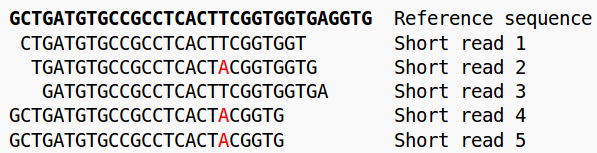
\includegraphics[width=\textwidth]{c2_genomics/ngs_reads_seq_01.png}
  \end{figure}
\end{frame}

\begin{frame}
  \frametitle{测序 | 第二代 | 简介}
  \begin{block}{Roche公司的454技术}
  \begin{itemize}
    \item 1996年,波尔·尼伦和穆斯塔法·罗纳吉,焦磷酸测序(pyrosequencing)
    \item 2004/2005年,商业化测序仪
    \item 2009年,百万条、200-400bp
  \end{itemize}
  \end{block}
  \pause
  \begin{block}{Illumina公司的Solexa技术}
  \begin{itemize}
    \item 2006年,商业化测序仪
    \item 2009年,上亿条、50-100bp
  \end{itemize}
  \end{block}
  \pause
  \begin{block}{ABI公司的SOLiD技术}
  \begin{itemize}
    \item 2006/2007年,商业化测序仪
  \end{itemize}
  \end{block}
\end{frame}

\begin{frame}
  \frametitle{测序 | 第二代 | Roche/454}
  \begin{block}{焦磷酸测序}
焦磷酸测序(pyrosequencing)是一种基于聚合原理的DNA测序方法,它依赖于核苷酸掺入中焦磷酸盐的释放,而非双脱氧三磷酸核苷酸参与的链终止反应。\\
\vspace{1em}
Pyrosequencing技术是由4种酶催化的同一反应体系中的酶级联化学发光反应。在每一轮测序中,只加入一种dNTP,若该dNTP与模板配对,聚合酶就可以将其掺入到引物链中并释放出等摩尔数的焦磷酸基团(PPi)。PPi可最终转化为可见光信号,并由PyrogramTM转化为一个峰值。每个峰值的高度与反应中掺入的核苷酸数目成正比。然后加入下一种dNTP,继续DNA链的合成。
  \end{block}
\end{frame}

\begin{frame}
  \frametitle{测序 | 第二代 | Roche/454}
  \begin{figure}
    \centering
    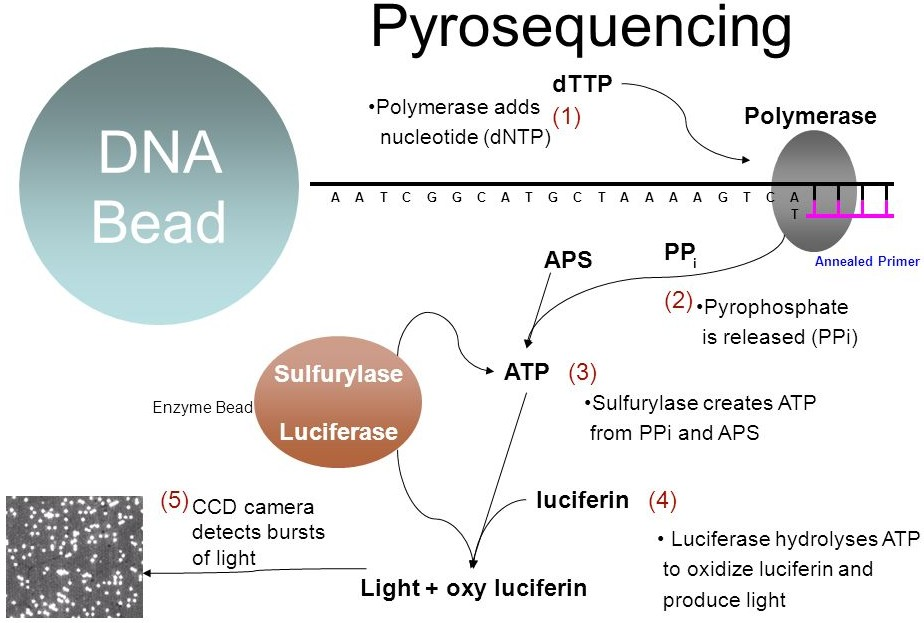
\includegraphics[width=0.9\textwidth]{c2_genomics/sequencing_pyro_02.jpg}
  \end{figure}
\end{frame}

\begin{frame}
  \frametitle{基因组学 | 测序 | 第二代 | Roche/454}
  \begin{block}{emPCR}
emPCR(乳液PCR)主要通过将水相PCR溶液(包含引物、聚合酶、核苷酸和待扩增DNA)与油混合,创建一种微小的悬浮水滴乳液。每个液滴都作为其自身PCR的“反应器”,从而创造了平行反应中的多个独立反应。\\
\vspace{1em}
emPCR(emulsion PCR)技术利用油包水(water-in-oil)结构作为PCR反应的微反应器,进行PCR扩增。emPCR最大的特点是可以形成数目庞大的独立反应空间以进行PCR扩增。其关键技术是“注水到油”,基本过程是在PCR反应前,将包含PCR所需反应成分的水溶液注入到高速旋转的油相表面,水溶液瞬间形成数以万计个被油相包裹的小液滴。这些小液滴就形成了PCR反应空间。
  \end{block}
\end{frame}

\begin{frame}
  \frametitle{测序 | 第二代 | Roche/454}
  \begin{figure}
    \centering
    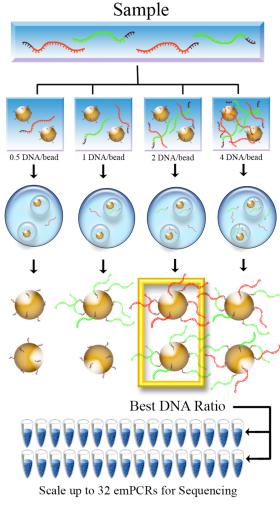
\includegraphics[width=0.36\textwidth]{c2_genomics/sequencing_empcr_01.jpg}
    \qquad
    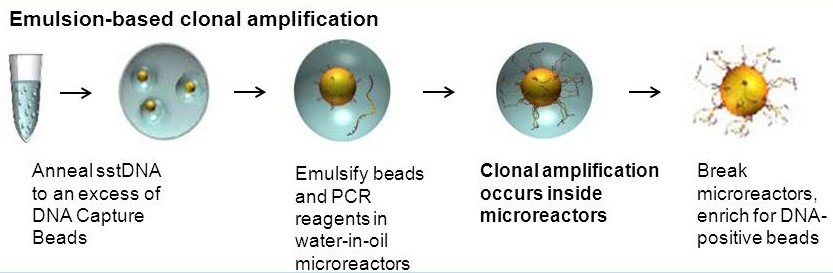
\includegraphics[angle=270,origin=r,width=0.18\textwidth]{c2_genomics/sequencing_empcr_05.jpg}
  \end{figure}
\end{frame}

\begin{frame}
  \frametitle{测序 | 第二代 | Roche/454}
  \begin{block}{概述}
在测序时,使用了一种叫做“Pico TiterPlate”(PTP)的平板,它含有160多万个由光纤组成的孔,孔中载有化学发光反应所需的各种酶和底物。测序开始时,放置在四个单独的试剂瓶里的四种碱基,依照T、A、C、G的顺序依次循环进入PTP板,每次只进入一个碱基。如果发生碱基配对,就会释放一个焦磷酸。这个焦磷酸在各种酶的作用下,经过一个合成反应和一个化学发光反应,最终将荧光素氧化成氧化荧光素,同时释放出光信号。此反应释放出的光信号实时被仪器配置的高灵敏度CCD捕获到。有一个碱基和测序模板进行配对,就会捕获到一分子的光信号;由此一一对应,就可以准确、快速地确定待测模板的碱基序列。
  \end{block}
\end{frame}

\begin{frame}
  \frametitle{测序 | 第二代 | Roche/454}
  \begin{figure}
    \centering
    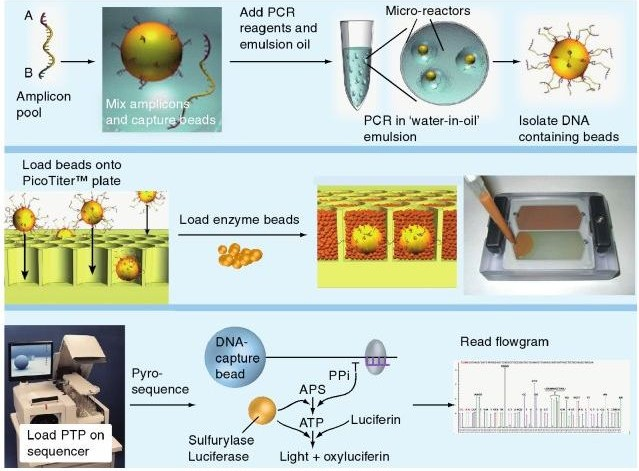
\includegraphics[width=0.9\textwidth]{c2_genomics/sequencing_454_01.jpg}
  \end{figure}
\end{frame}

\begin{frame}
  \frametitle{测序 | 第二代 | Roche/454}
  \begin{block}{优点}
    \begin{itemize}
      \item 读长长,使得后继的序列拼接工作更加高效、准确
      \item 速度快,一个测序反应耗时10个小时,获得4-6亿个碱基对
      \item 特别适合从头拼接和宏基因组学应用,多用于新的细菌基因组
    \end{itemize}
  \end{block}
  \pause
  \begin{block}{缺点}
    \begin{itemize}
      \item 无法准确测量同聚物的长度,所以检测插入缺失突变的误差率高
      \item 通量小且费用高
      \item 对重测序来说太贵,不适合
    \end{itemize}
  \end{block}
\end{frame}

\begin{frame}
  \frametitle{测序 | 第二代 | \textcolor{red}{Illumina/Solexa}}
  \begin{block}{边合成边测序}
边合成边测序(sequencing by synthesis,SBS):以DNA单链为模板,在合成互补链的时候,利用带荧光标记的dNTP发出不同的荧光来确定碱基类型。
  \end{block}
\end{frame}

\begin{frame}
  \frametitle{测序 | 第二代 | Illumina/Solexa}
  \begin{figure}
    \centering
    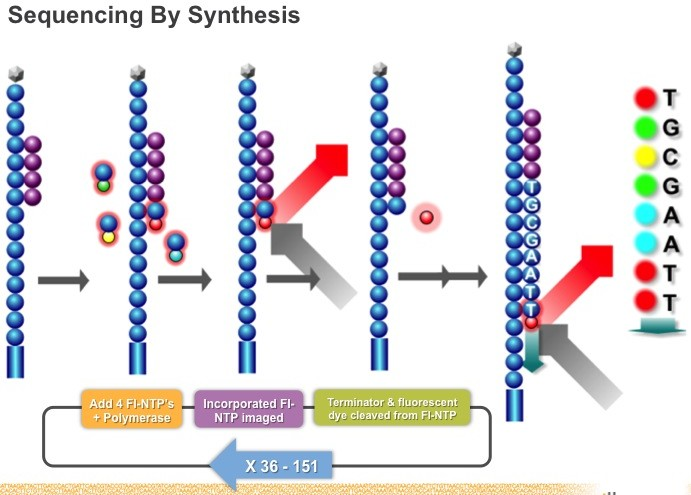
\includegraphics[width=0.9\textwidth]{c2_genomics/sequencing_sbs_01.jpg}
  \end{figure}
\end{frame}

\begin{frame}
  \frametitle{测序 | 第二代 | Illumina/Solexa}
  \begin{figure}
    \centering
    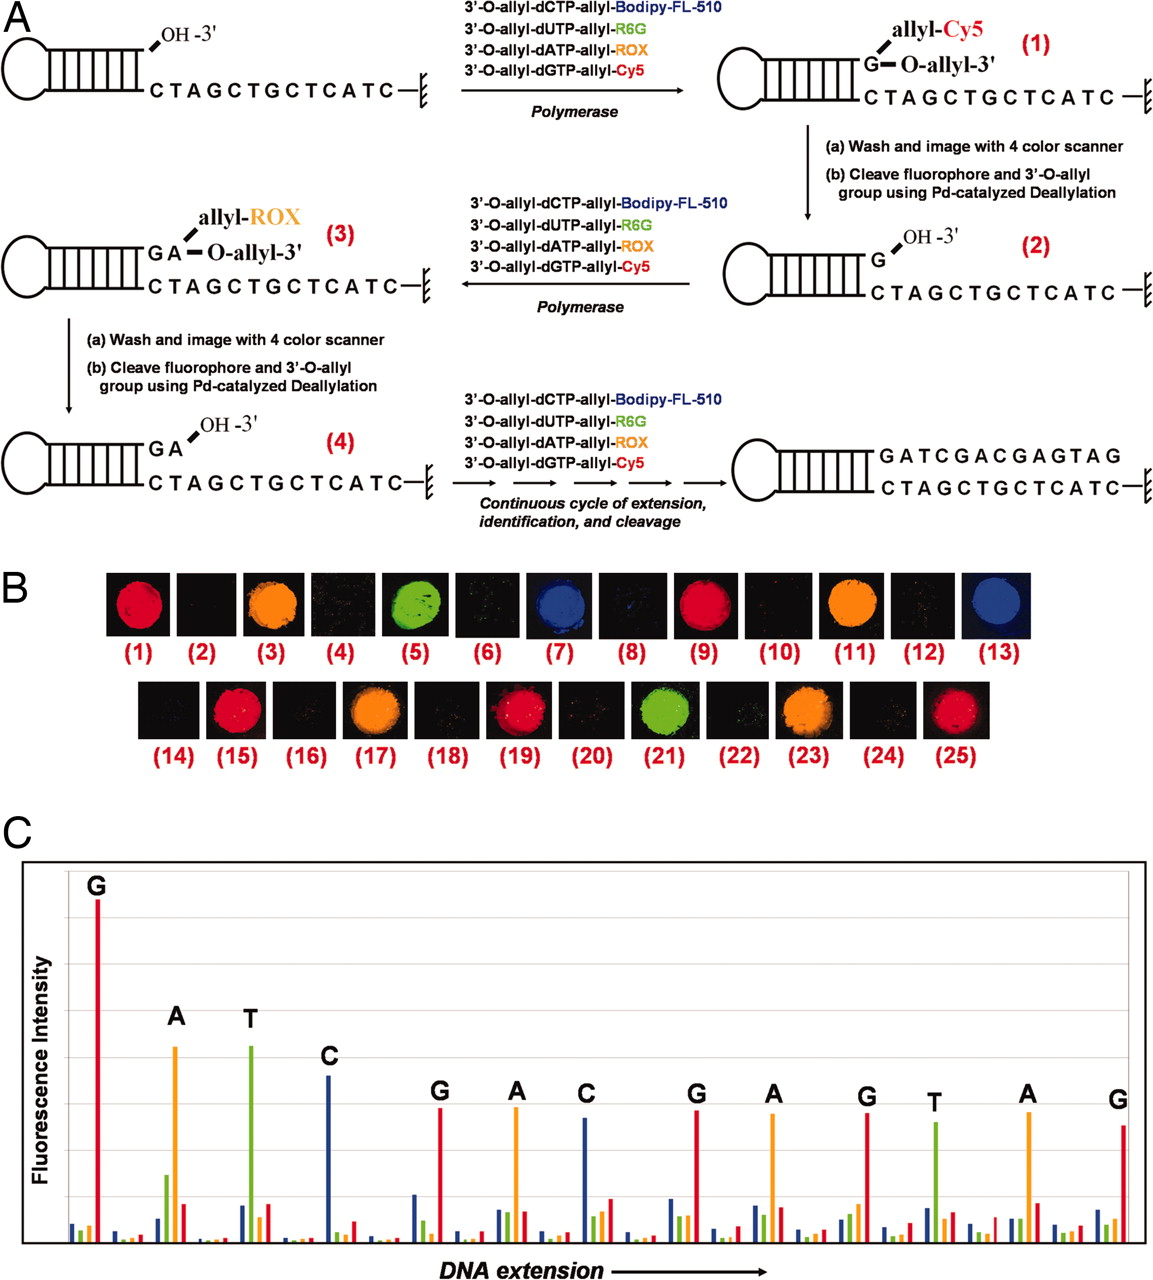
\includegraphics[width=0.59\textwidth]{c2_genomics/sequencing_sbs_04.jpg}
  \end{figure}
\end{frame}

\begin{frame}
  \frametitle{测序 | 第二代 | \textcolor{red}{Illumina/Solexa}}
  \begin{block}{桥式扩增}
桥式扩增(bridge amplification):随机打断的单链DNA片段通过两端接头与寡核苷酸的互补固定在芯片表面,形成桥形结构,之后以寡核苷酸为引物进行PCR扩增,得到单克隆的DNA簇群。
  \end{block}
\end{frame}

\begin{frame}
  \frametitle{测序 | 第二代 | Illumina/Solexa}
  \begin{figure}
    \centering
    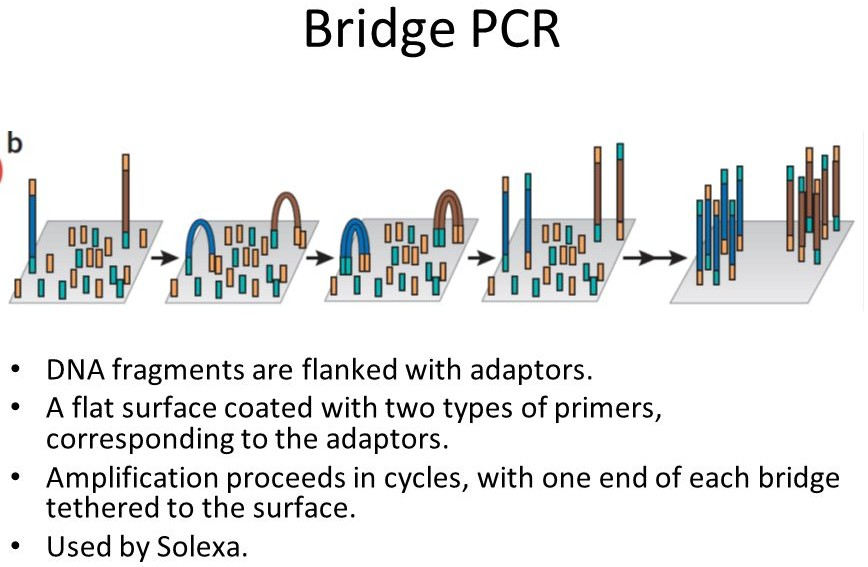
\includegraphics[width=0.9\textwidth]{c2_genomics/sequencing_bridge_01.jpg}
  \end{figure}
\end{frame}

\begin{frame}
  \frametitle{测序 | 第二代 | Illumina/Solexa}
  \begin{figure}
    \centering
    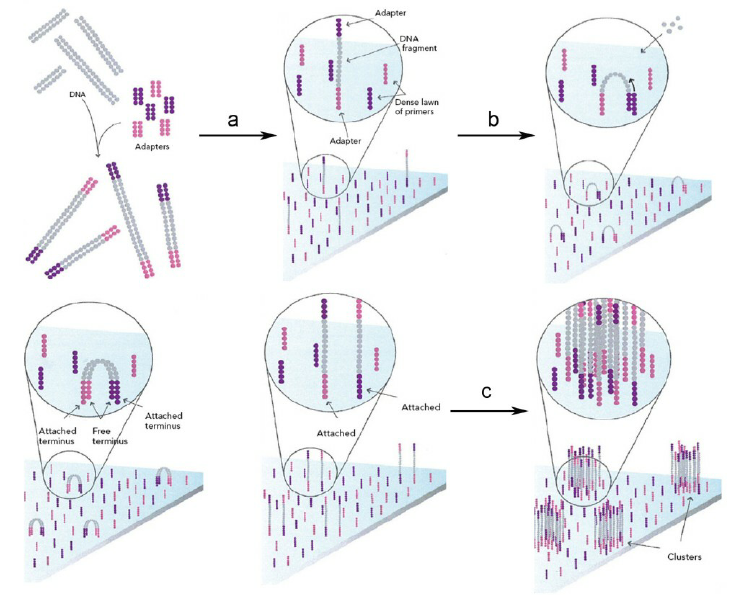
\includegraphics[width=0.8\textwidth]{c2_genomics/sequencing_bridge_02.png}
  \end{figure}
\end{frame}

\begin{frame}
  \frametitle{测序 | 第二代 | \textcolor{red}{Illumina/Solexa}}
  \begin{block}{概述}
这种测序技术通过将基因组DNA的随机片断附着到光学透明的表面,这些DNA片断通过延长和桥梁扩增,形成了具有数以亿计cluster的Flowcell,每个cluster具有约1000拷贝的相同DNA模板,然后用4种末端被封闭的不同荧光标记的碱基进行边合成边测序。这种新方法确保了高精确度和真实的一个碱基接一个碱基的测序,排除了序列方面的特殊错误,能够测序同聚物和重复序列。
  \end{block}
\end{frame}

\begin{frame}
  \frametitle{测序 | 第二代 | Illumina/Solexa}
  \begin{figure}
    \centering
    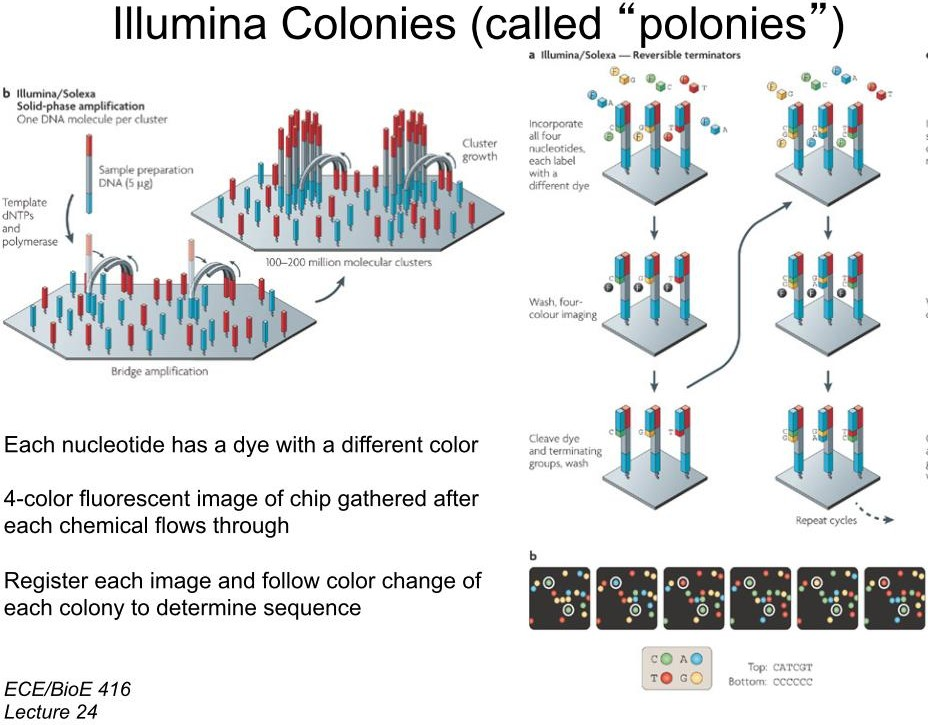
\includegraphics[width=0.82\textwidth]{c2_genomics/sequencing_ill_05.jpg}
  \end{figure}
\end{frame}

\begin{frame}
  \frametitle{测序 | 第二代 | Illumina/Solexa}
  \begin{figure}
    \centering
    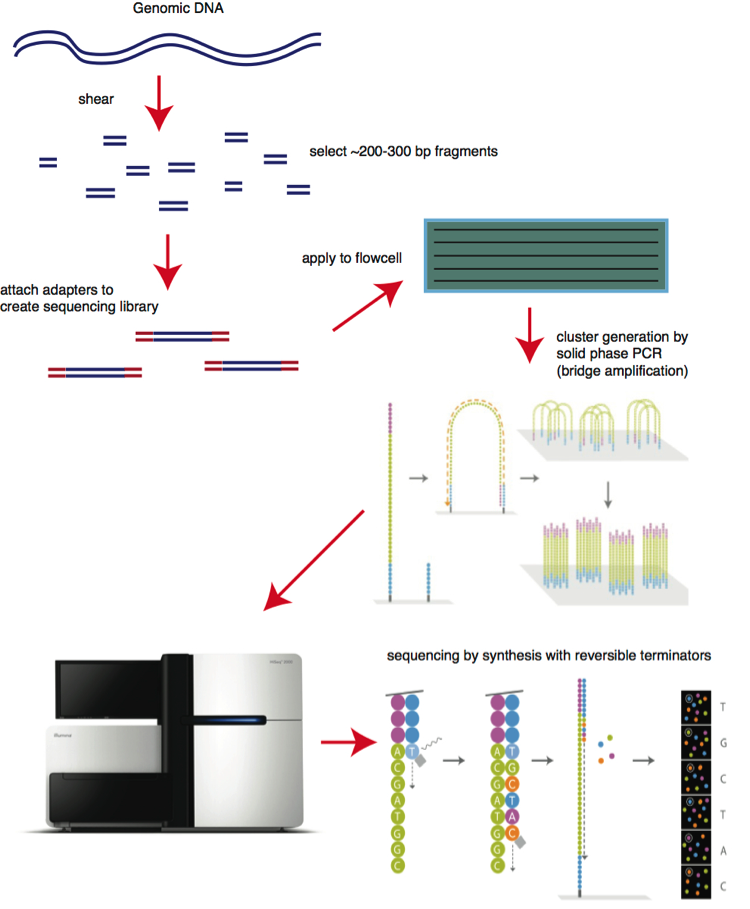
\includegraphics[width=0.52\textwidth]{c2_genomics/sequencing_ill_01.png}
  \end{figure}
\end{frame}

\begin{frame}
  \frametitle{测序 | 第二代 | Illumina/Solexa}
  \begin{block}{优点}
    \begin{itemize}
      \item 通量大
      \item 测序方式灵活
      \item 分析软件多样化
    \end{itemize}
  \end{block}
  \pause
  \begin{block}{缺点}
    \begin{itemize}
      \item 样本制备过程复杂
      \item 样本要求相对较高
    \end{itemize}
  \end{block}
\end{frame}

\begin{frame}
  \frametitle{测序 | 第二代 | ABI/SOLiD}
  \begin{block}{边连接边测序}
边连接边测序(sequencing by ligation),基于连接酶法,即利用DNA连接酶在连接过程之中测序。
  \end{block}
\end{frame}

\begin{frame}
  \frametitle{测序 | 第二代 | ABI/SOLiD}
  \begin{figure}
    \centering
    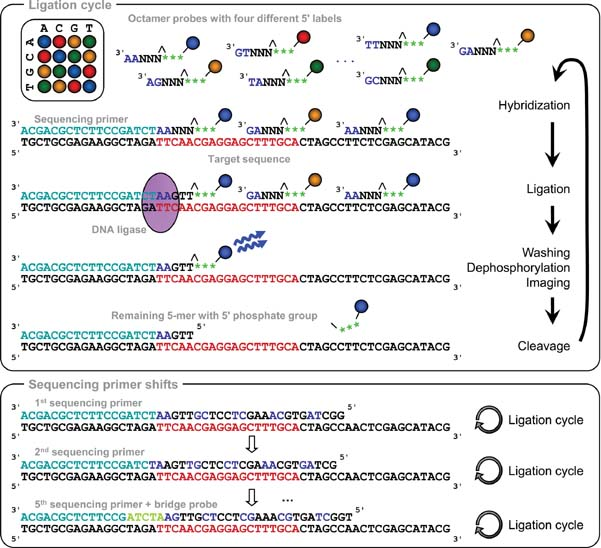
\includegraphics[width=0.7\textwidth]{c2_genomics/sequencing_sbl_01.jpg}
  \end{figure}
\end{frame}

\begin{frame}
  \frametitle{测序 | 第二代 | ABI/SOLiD}
  \begin{block}{概述}
SOLiD连接反应的底物是8碱基单链荧光探针混合物(3'-XXnnnzzz-5'),其中第1和第2位碱基(XX)上的碱基是确定的,并根据种类的不同在6-8位(zzz)上加上CY5、Texas Red、CY3、6-FAM四种不同的荧光标记。这是SOLiD的独特测序法,两个碱基确定一个荧光信号,相当于一次能决定两个碱基,因此也称为两碱基测序法。当荧光探针能够与DNA模板链配对而连接上时,就会发出代表第1、2位碱基的荧光信号。在记录下荧光信号后,通过化学方法在第5和第6位碱基之间进行切割,这样就能移除荧光信号,以便进行下一个位置的测序。这种测序方法每次测序的位置都相差5位:即第一次是第1、2位,第二次是第6、7位……在测到末尾后,要将新合成的链变性,洗脱。接着用引物n-1进行第二轮测序。引物n-1与引物n的区别是,二者在与接头配对的位置上相差一个碱基。也即是,通过引物n-1在引物n的基础上将测序位置往3'端移动一个碱基位置,因而就能测定第0、1位和第5、6位……第二轮测序完成,依此类推,直至第五轮测序,最终可以完成所有位置的碱基测序,并且每个位置的碱基均被检测了两次。
  \end{block}
\end{frame}

\begin{frame}
  \frametitle{测序 | 第二代 | ABI/SOLiD}
  \begin{figure}
    \centering
    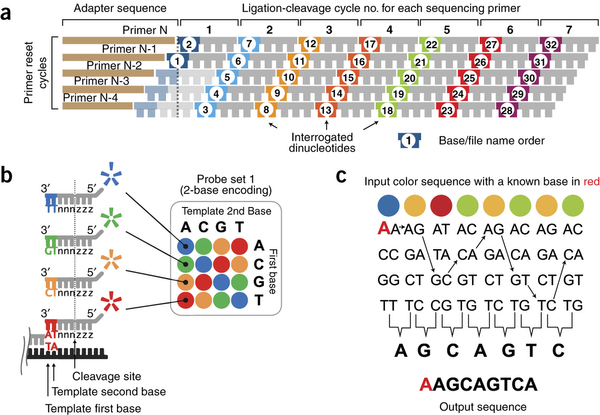
\includegraphics[width=0.9\textwidth]{c2_genomics/sequencing_sbl_02.jpg}
  \end{figure}
\end{frame}

\begin{frame}
  \frametitle{测序 | 第二代 | ABI/SOLiD}
  \begin{figure}
    \centering
    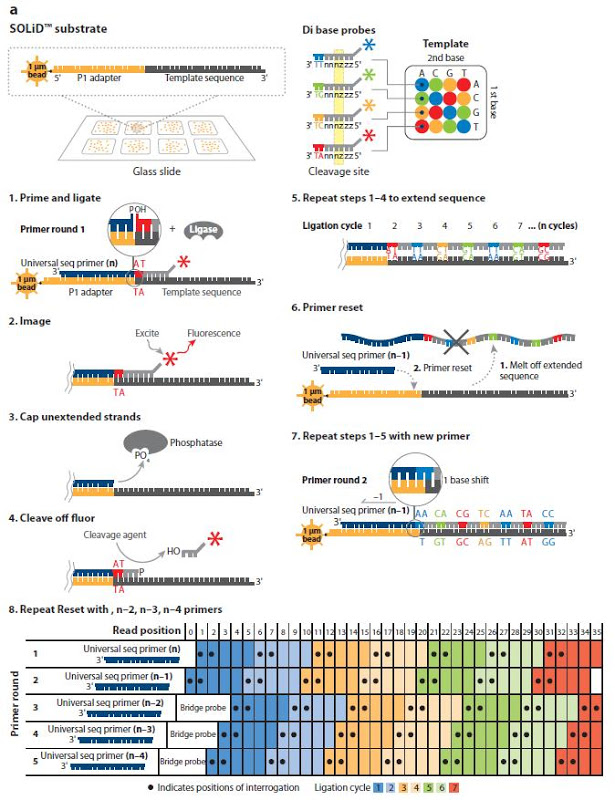
\includegraphics[width=0.48\textwidth]{c2_genomics/sequencing_solid_02.jpg}
  \end{figure}
\end{frame}

\begin{frame}
  \frametitle{测序 | 第二代 | ABI/SOLiD}
  \begin{figure}
    \centering
    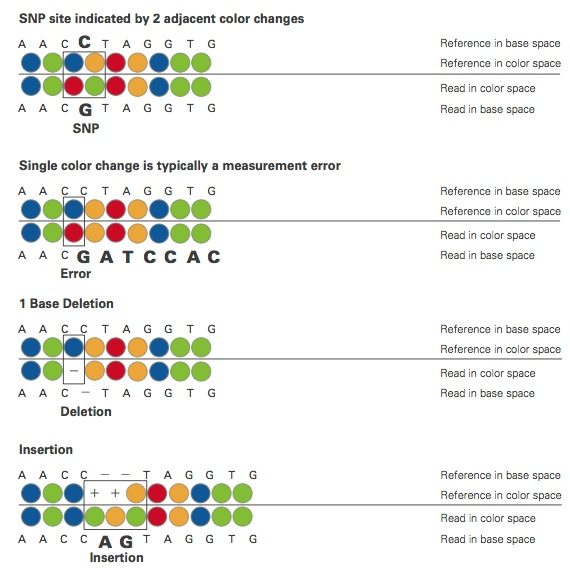
\includegraphics[width=0.62\textwidth]{c2_genomics/sequencing_sbl_04.jpg}
  \end{figure}
\end{frame}

\begin{frame}
  \frametitle{测序 | 第二代 | ABI/SOLiD}
  \begin{figure}
    \centering
    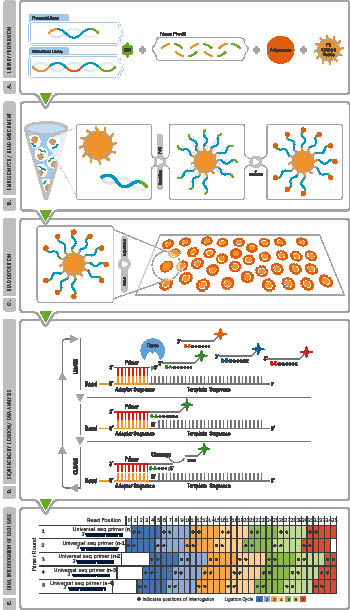
\includegraphics[width=0.38\textwidth]{c2_genomics/sequencing_solid_01.jpg}
  \end{figure}
\end{frame}

\begin{frame}
  \frametitle{测序 | 第二代 | ABI/SOLiD}
  \begin{block}{优点}
    \begin{itemize}
      \item 高准确性,每个DNA碱基检测2次,增加了序列读取的准确性
    \end{itemize}
  \end{block}
  \pause
  \begin{block}{缺点}
    \begin{itemize}
      \item 运行时间长,检测碱基替换突变的误差率高
    \end{itemize}
  \end{block}
\end{frame}

\begin{frame}
  \frametitle{测序 | 第2.5代 | 离子半导体测序}
  \begin{block}{概述}
    Ion Torrent(Ion semiconductor sequencing)是一种基于半导体芯片的新一代革命性测序技术,通过检测H+信号的变化来获得序列碱基信息。该技术使用了一种布满小孔的高密度半导体芯片,一个小孔就是一个测序反应池,芯片置于一个离子敏感层和离子感受器之上。当DNA聚合酶把核苷酸聚合到延伸中的DNA链上时,会释放出一个氢离子,反应池中的pH发生改变,位于池下的离子感受器感受到H+离子信号,H+离子信号再直接转化为数字信号,从而读出DNA序列。
  \end{block}
\end{frame}

\begin{frame}
  \frametitle{测序 | 第2.5代 | 离子半导体测序}
  \begin{figure}
    \centering
    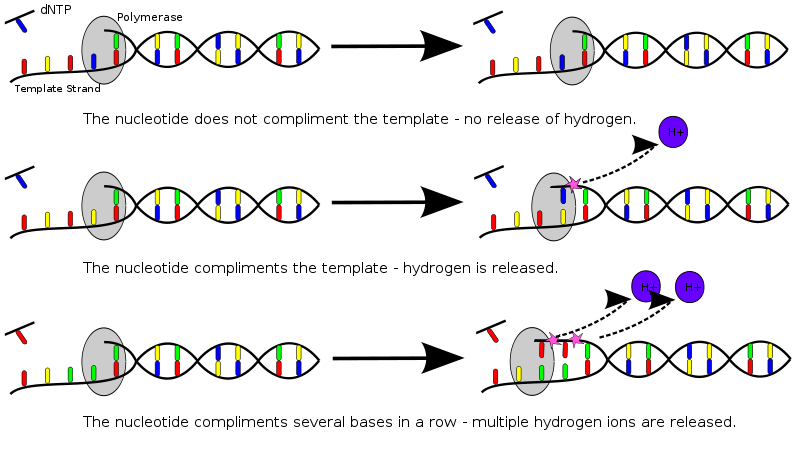
\includegraphics[width=0.9\textwidth]{c2_genomics/sequencing_ion_01.png}
  \end{figure}
\end{frame}

\begin{frame}
  \frametitle{测序 | 第2.5代 | 离子半导体测序}
  \begin{figure}
    \centering
    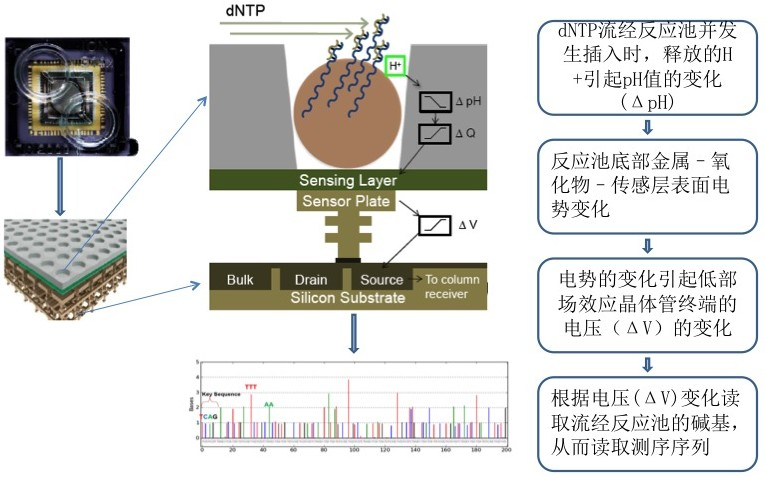
\includegraphics[width=0.9\textwidth]{c2_genomics/sequencing_ion_07.jpg}
  \end{figure}
\end{frame}

\begin{frame}
  \frametitle{测序 | 第2.5代 | 离子半导体测序}
  \begin{figure}
    \centering
    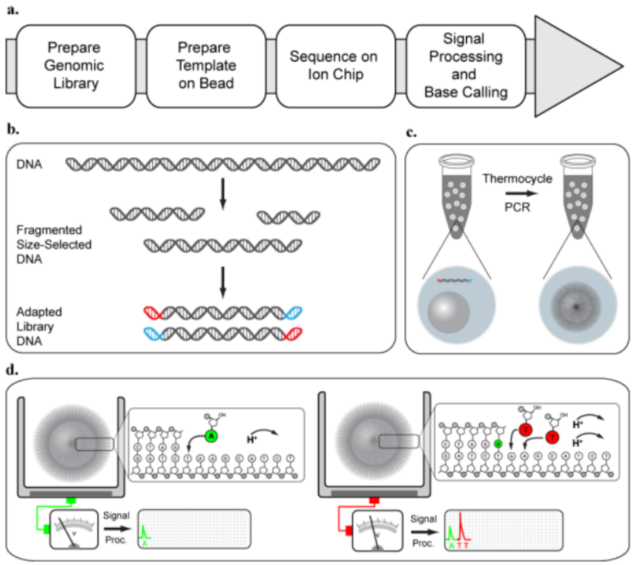
\includegraphics[width=0.7\textwidth]{c2_genomics/sequencing_ion_03.png}
  \end{figure}
\end{frame}

\begin{frame}
  \frametitle{测序 | 第2.5代 | 离子半导体测序}
  \begin{figure}
    \centering
    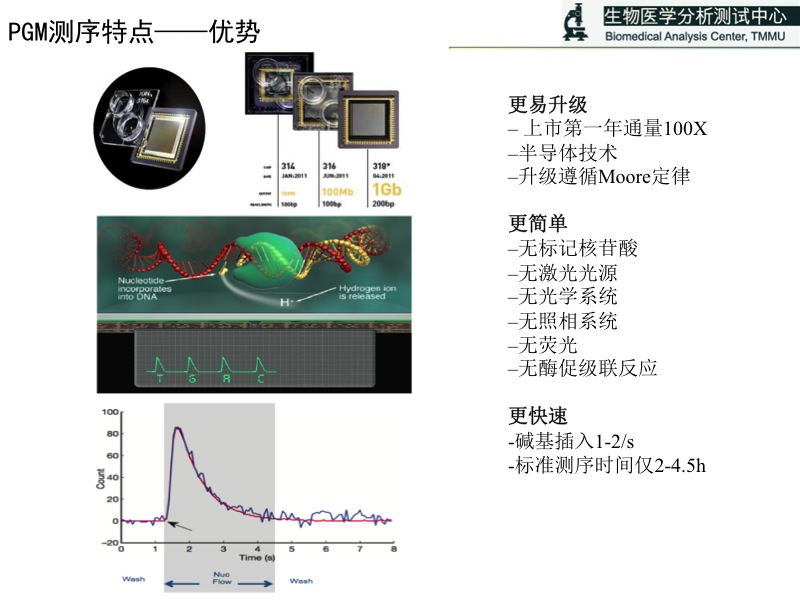
\includegraphics[width=0.85\textwidth]{c2_genomics/sequencing_ion_08.jpg}
  \end{figure}
\end{frame}

\begin{frame}
  \frametitle{测序 | 第2.5代 | 离子半导体测序}
  \begin{block}{优缺点}
Ion Torrent相比于其他测序技术来说,不需要昂贵的物理成像等设备,因此,成本相对来说会低,体积也会比较小,同时操作也要更为简单,速度也相当快速,除了2天文库制作时间,整个上机测序可在2-3.5小时内完成,不过整个芯片的通量并不高,目前是10G左右,但非常适合小基因组和外显子验证的测序。\\
\vspace{1em}
Ion Torrent的化学测序原理自然简单,无修饰的核苷酸、无激光器或光学检测设备,因而可达到极小的测序偏差和出色的测序覆盖均衡度。
  \end{block}
\end{frame}

\begin{frame}
  \frametitle{测序 | 第二代 | \alert{比较}}
  \begin{figure}
    \centering
    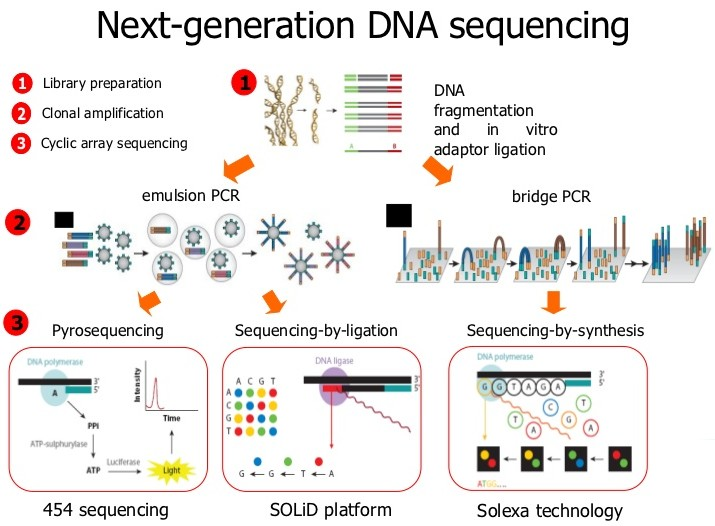
\includegraphics[width=0.88\textwidth]{c2_genomics/sequencing_ngs_01.jpg}
  \end{figure}
\end{frame}

\begin{frame}
  \frametitle{测序 | 第二代 | \alert{比较}}
  \begin{figure}
    \centering
    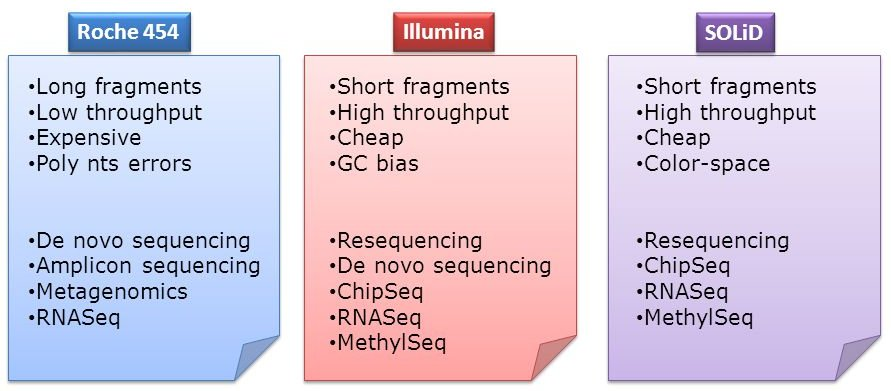
\includegraphics[width=0.9\textwidth]{c2_genomics/sequencing_compare_00.jpg}
  \end{figure}
\end{frame}

\subsection{第三代测序技术}
\begin{frame}
  \frametitle{测序 | 第三代 | 简介}
  \begin{block}{单分子测序}
测序过程无需进行PCR扩增。
  \end{block}
\end{frame}

\begin{frame}
  \frametitle{测序 | 第三代 | tSMS}
  \begin{block}{概述}
真正的单分子测序(Helicos True Single Molecule Sequencing)。待测DNA被随机打断成小片段,在每个小片段(~200bp)的末端加上poly-dA,并于玻璃芯片上随机固定多个poly-dT引物,其末端皆带有荧光标记,以利于精确定位。首先,将小片段DNA模板与检测芯片上的poly-dT引物进行杂交并精确定位,然后逐一加入荧光标记的末端终止子。这个终止子与Illumina的终止子可不一样,不是四色的,是单色的,也就是说所有终止子都标有同一种染料。在掺入了单个荧光标记的核苷酸后,洗涤,单色成像,之后切开荧光染料和抑制基团,洗涤,加帽,允许下一个核苷酸的掺入。通过掺入、检测和切除的反复循环,即可实时读取大量序列。最后以软件系统辅助,可分析出完整的核酸序列。
  \end{block}
\end{frame}

\begin{frame}
  \frametitle{测序 | 第三代 | tSMS}
  \begin{figure}
    \centering
    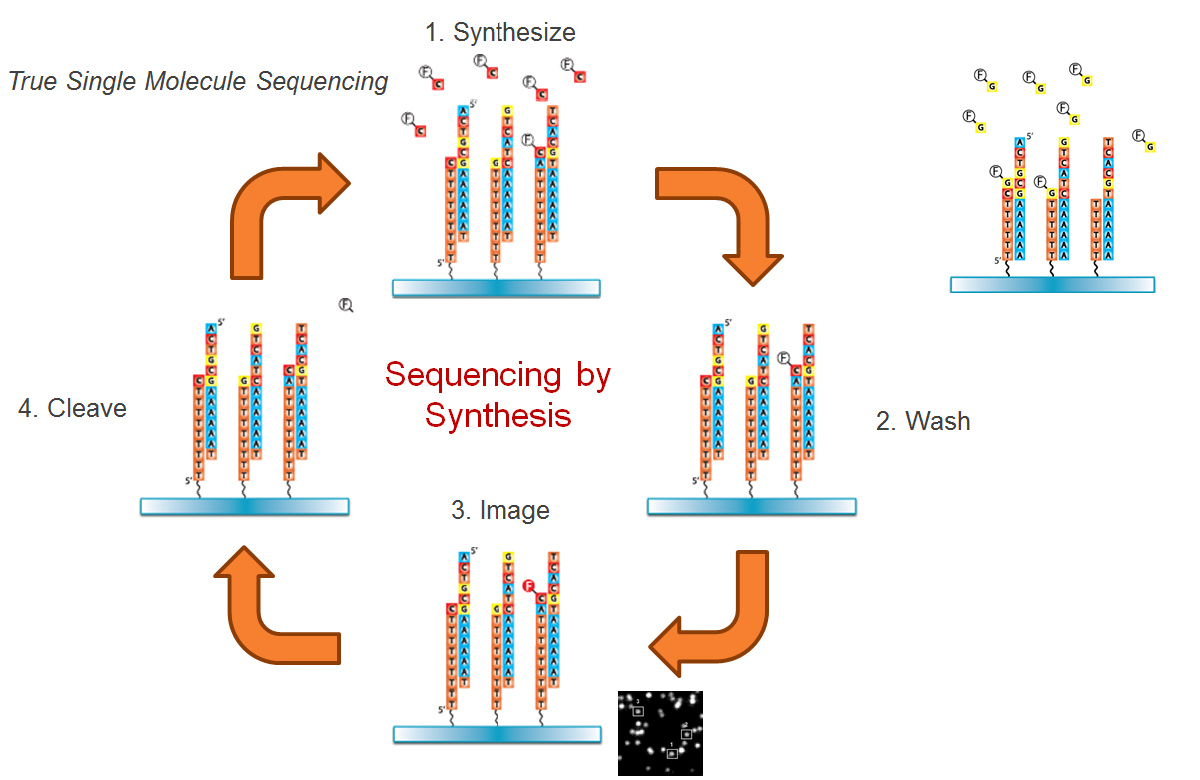
\includegraphics[width=0.9\textwidth]{c2_genomics/sequencing_sms_01.jpg}
  \end{figure}
\end{frame}

\begin{frame}
  \frametitle{测序 | 第三代 | tSMS}
  \begin{figure}
    \centering
    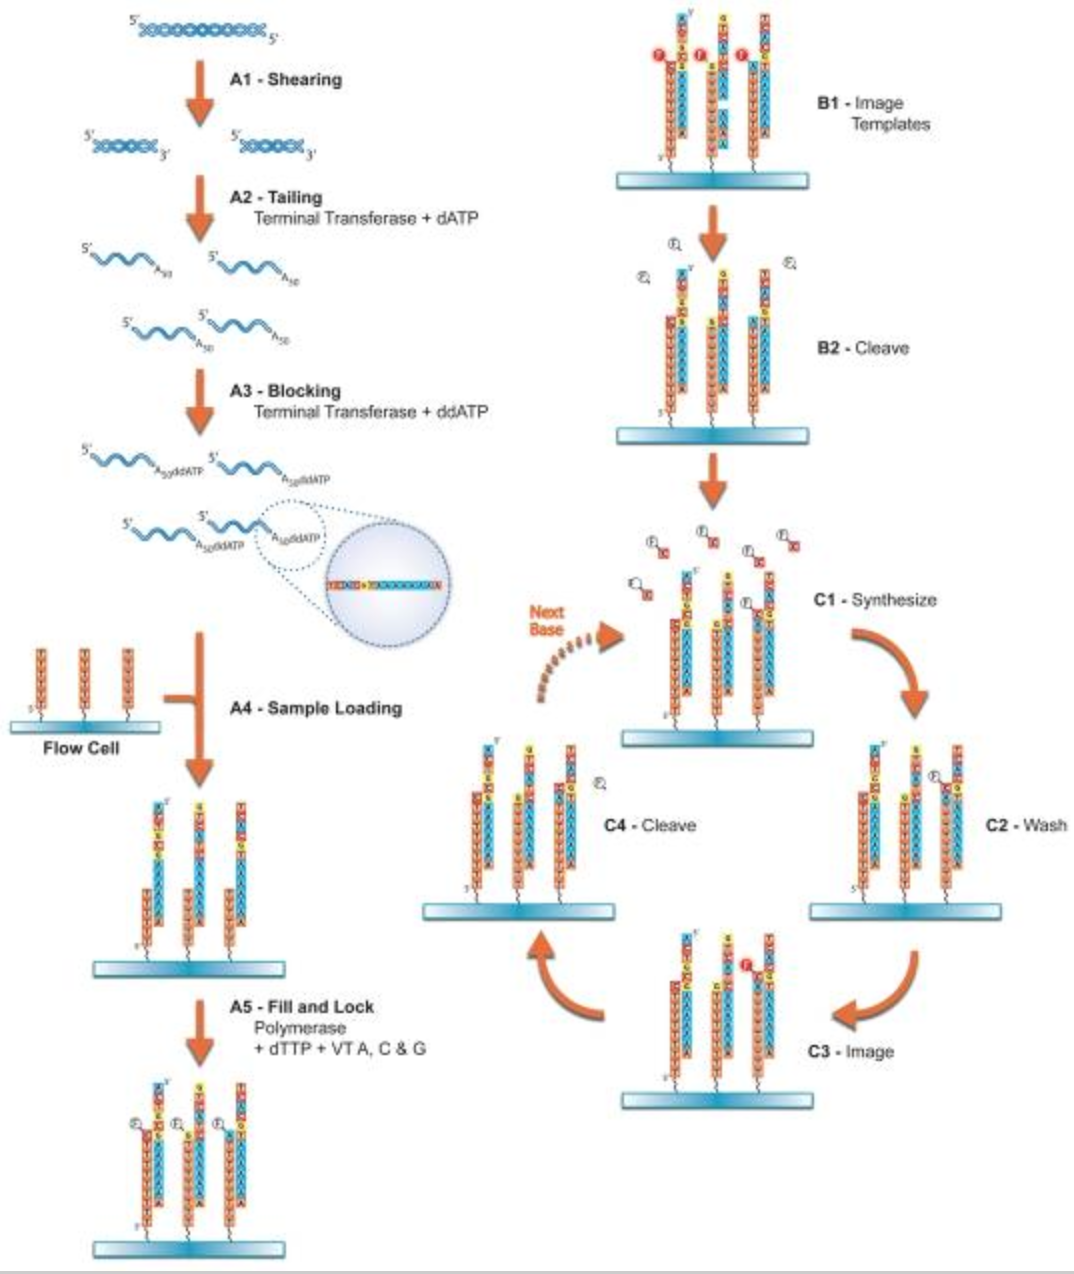
\includegraphics[width=0.5\textwidth]{c2_genomics/sequencing_sms_04.png}
  \end{figure}
\end{frame}

\begin{frame}
  \frametitle{测序 | 第三代 | tSMS}
  \begin{block}{优缺点}
    真正的单分子测序,无需前期扩增,不引入偏向性;特别适合RNA-Seq或RNA直接测序的应用,因为它\textcolor{red}{能直接测序RNA模板},而无需将其转化成cDNA。检测碱基替换突变的误差率非常低,~0.2\%。\\
\vspace{1em}
缺点: 错误率高,Insertion 1.5\%,Deletion 3.0\%;Heliscope在面对同聚物时也会遇到一些困难,但可以通过二次测序提高准确度;由于在合成中可能掺有未标记的碱基,因此其最主要的错误来源是缺失。
  \end{block}
\end{frame}

\begin{frame}
  \frametitle{测序 | 第三代 | \alert{SMRT}}
  \begin{block}{概述}
PacBio SMRT(single molecule real time sequencing)技术也应用了边合成边测序的思想,并以SMRT芯片为测序载体。\\
\vspace{1em}
基本原理是:DNA聚合酶和模板结合,4色荧光标记4种碱基(即是dNTP),在碱基配对阶段,不同碱基的加入,会发出不同光,根据光的波长与峰值可判断进入的碱基类型。\\
\vspace{1em}
DNA聚合酶是实现超长读长的关键之一,读长主要跟酶的活性保持有关,它主要受激光对其造成的损伤所影响。
  \end{block}
\end{frame}

\begin{frame}
  \frametitle{测序 | 第三代 | SMRT}
  \begin{block}{概述}
    PacBio SMRT技术的一个关键是怎样将反应信号与周围游离碱基的强大荧光背景区别出来。它们利用的是ZMW(Zero Mode Waveguide,零模波导孔)原理,如同微波炉壁上可看到的很多密集小孔。小孔直径有考究,如果直径大于微波波长,能量就会在衍射效应的作用下穿透面板而泄露出来,从而与周围小孔相互干扰。如果孔径小于波长,能量不会辐射到周围,而是保持直线状态(光衍射的原理),从而可起保护作用。同理,在一个反应管(SMRT Cell,单分子实时反应孔)中有许多这样的圆形纳米小孔,即ZMW(零模波导孔),外径100多纳米,比检测激光波长小(数百纳米),激光从底部打上去后不能穿透小孔进入上方溶液区,能量被限制在一个小范围(体积$20 \times 10^{-21}L$ )里,正好足够覆盖需要检测的部分,使得信号仅来自这个小反应区域,孔外过多游离核苷酸单体依然留在黑暗中,从而实现将背景降到最低。
  \end{block}
\end{frame}

\begin{frame}
  \frametitle{测序 | 第三代 | SMRT}
  \begin{figure}
    \centering
    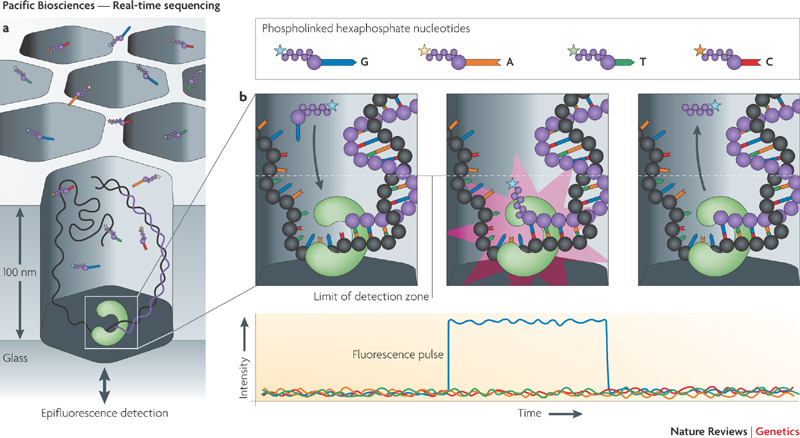
\includegraphics[width=0.9\textwidth]{c2_genomics/sequencing_smrt_01.jpg}
  \end{figure}
\end{frame}

\begin{frame}
  \frametitle{测序 | 第三代 | SMRT}
  \begin{block}{优缺点}
可以通过检测相邻两个碱基之间的测序时间,来检测一些碱基修饰情况,即如果碱基存在修饰,则通过聚合酶时的速度会减慢,相邻两峰之间的距离增大,可以通过这个来\textcolor{red}{直接检测甲基化}等信息。\\
\vspace{1em}
SMRT技术的测序速度很快,每秒约10个dNTP。读长长。无需PCR扩增,也避免了由此带来的bias。需要的样品量很少,样品制备时间花费少。通量灵活,时间快。可以远程快速获取数据和选择测序参数。\\
\vspace{1em}
SMRT技术的测序错误率比较高(这几乎是目前单分子测序技术的通病),达到15\%,但好在它的出错是随机的,并不会像第二代测序技术那样存在测序错误的偏向,因而可以通过多次测序来进行有效的纠错。
  \end{block}
\end{frame}

\begin{frame}
  \frametitle{测序 | 第三代 | SMRT}
  \begin{figure}
    \centering
    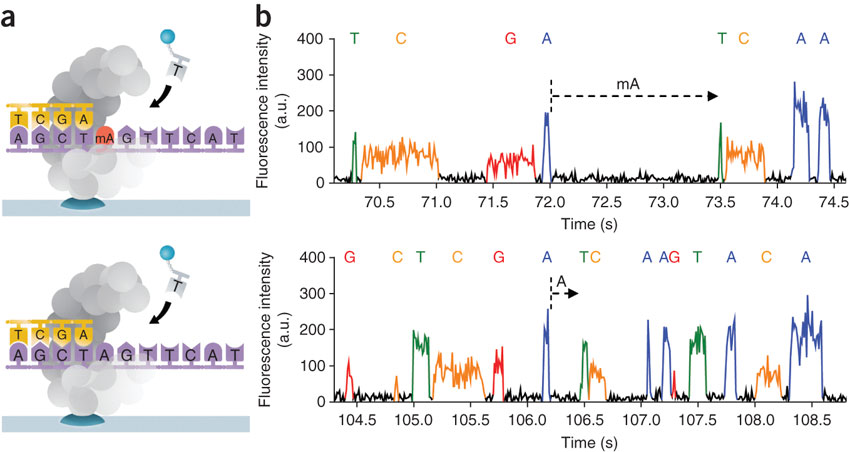
\includegraphics[width=0.9\textwidth]{c2_genomics/sequencing_smrt_03.jpg}
  \end{figure}
\end{frame}

\begin{frame}
  \frametitle{测序 | 第三代 | FRET}
  \begin{block}{概述}
VisiGen基于荧光共振能量转移(FRET,Fluorescence Resonance Energy Transfer)的DNA测序技术。将标记了荧光供体基团的DNA聚合酶分子固定在载玻片上;再加含模板、引物、四种dNTP(其磷酸上标记特异的荧光受体基团)的测序缓冲液。\\
\vspace{1em}
测序延伸反应开始,带荧光受体基团的dNTP靠近含荧光供体基团的聚合酶,使后者释放能量,激发前者发出特异的荧光(即FRET信号),从而识别相应的碱基序列。当dNTP被加上后,荧光基团随磷酸离开,保证下一个dNTP能继续被加上。
  \end{block}
\end{frame}

\begin{frame}
  \frametitle{测序 | 第三代 | FRET}
  \begin{figure}
    \centering
    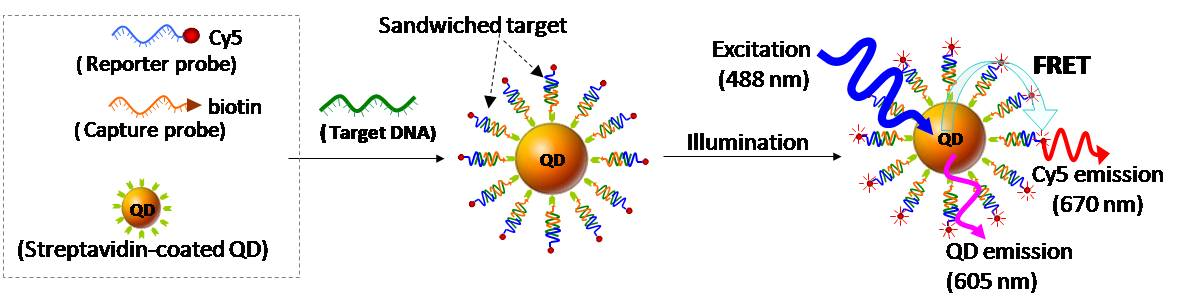
\includegraphics[width=0.9\textwidth]{c2_genomics/sequencing_fret_01.jpg}
  \end{figure}
\end{frame}

\begin{frame}
  \frametitle{测序 | 第三代 | \alert{纳米孔测序}}
  \begin{block}{概述}
Oxford Nanopore Technologies公司所开发的纳米单分子测序技术(Nanopore sequencing)与以往的测序技术皆不同,是基于电信号而不是光信号的测序技术。该技术的关键之一是,它们设计了一种特殊的纳米孔,孔内共价结合有分子接头。当DNA碱基通过纳米孔时,它们使电荷发生变化,从而短暂地影响流过纳米孔的电流强度(每种碱基所影响的电流变化幅度是不同的),灵敏的电子设备检测到这些变化从而鉴定所通过的碱基。
  \end{block}
\end{frame}

\begin{frame}
  \frametitle{测序 | 第三代 | 纳米孔测序}
  \begin{figure}
    \centering
    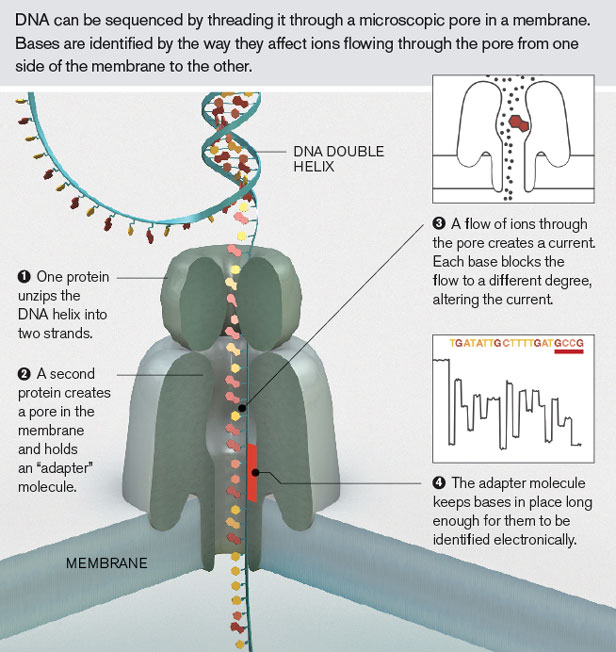
\includegraphics[width=0.6\textwidth]{c2_genomics/sequencing_nano_01.jpg}
  \end{figure}
\end{frame}

\begin{frame}
  \frametitle{测序 | 第三代 | 纳米孔测序}
  \begin{block}{优缺点}
纳米孔测序的主要特点是:读长很长,大约在几十kb,甚至100kb;错误率目前介于1\%至4\%,且是随机错误,而不是聚集在读段的两端;数据可实时读取;通量很高(30x人类基因组有望在一天内完成);起始DNA在测序过程中不被破坏;样品制备简单又便宜。理论上,它也\textcolor{red}{能直接测序RNA}。\\
\vspace{1em}
纳米孔单分子测序还有另外一大特点,它\textcolor{red}{能够直接读取出甲基化的胞嘧啶},而不必像传统方法那样对基因组进行bisulfite处理。这对于在基因组水平直接研究表观遗传相关现象有极大的帮助。并且该方法的测序准确性可达99.8\%,而且一旦发现测序错误也能较容易地进行纠正。
  \end{block}
\end{frame}

\begin{frame}
  \frametitle{测序 | 第三代 | 纳米孔测序}
  \begin{figure}
    \centering
    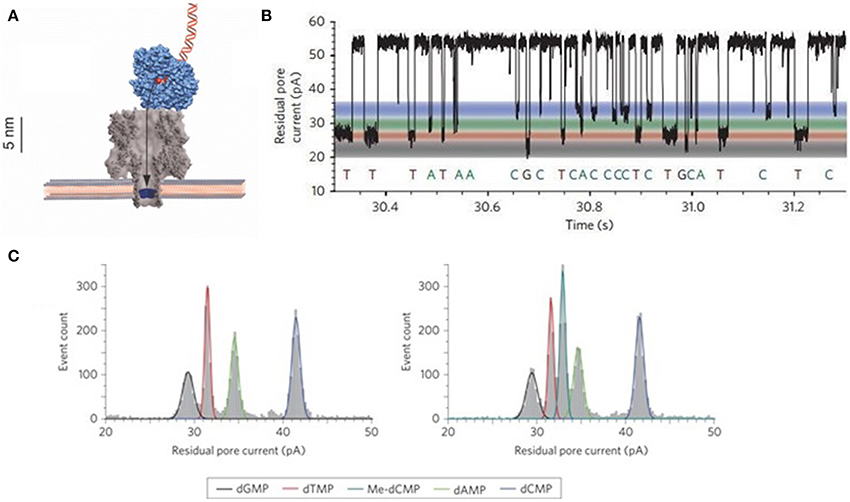
\includegraphics[width=\textwidth]{c2_genomics/sequencing_nano_02.jpg}
  \end{figure}
\end{frame}

\begin{frame}
  \frametitle{测序 | 第三代 | TEM}
  \begin{block}{概述}
以单链线性DNA为模板,以三种重元素标记、一种不标记的脱氧核苷酸为原料,合成其互补链,经透射电镜(TEM,Transmission electron microscopy)检测,则可见重元素标记,其互补链则可由点的大小和强度被分辨出来。
  \end{block}
\end{frame}

\begin{frame}
  \frametitle{测序 | 第三代 | TEM}
  \begin{figure}
    \centering
    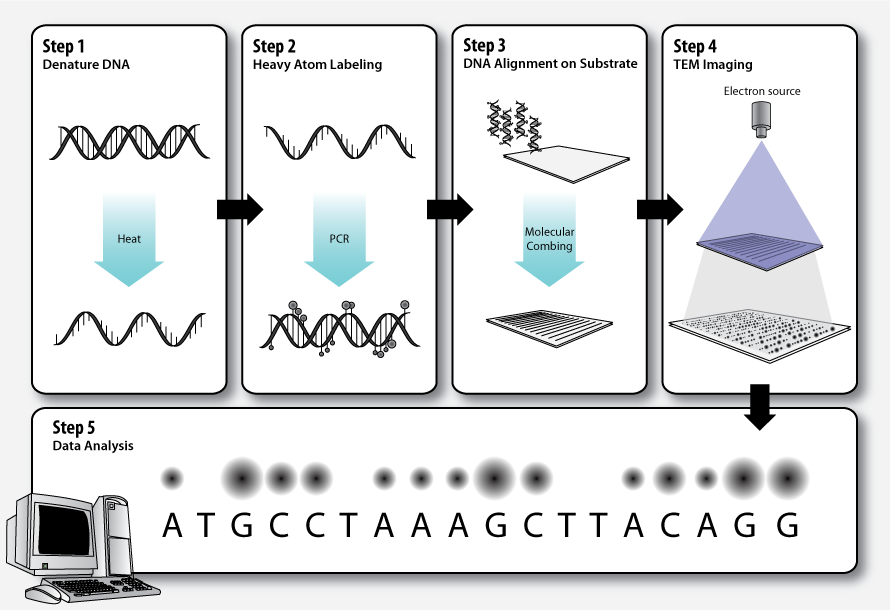
\includegraphics[width=0.9\textwidth]{c2_genomics/sequencing_tem_01.png}
  \end{figure}
\end{frame}

\begin{frame}
  \frametitle{测序 | 第三代 | SMRT, Nanopore}
  \begin{figure}
    \centering
    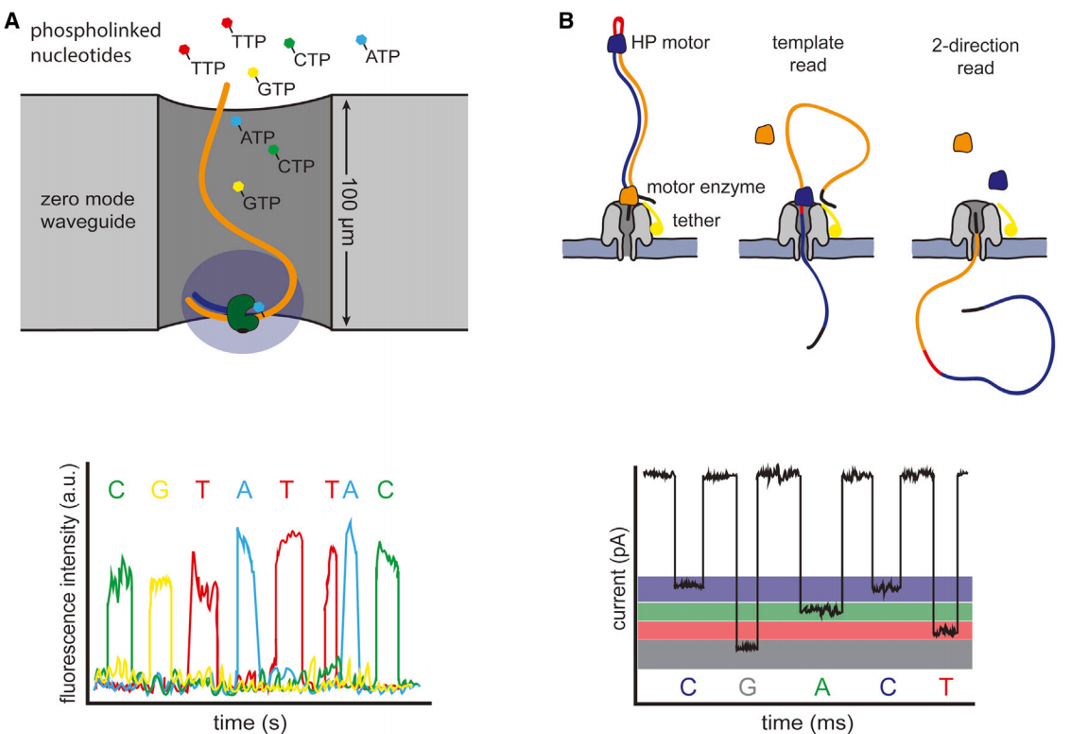
\includegraphics[width=0.9\textwidth]{c2_genomics/sequencing_smrt_nano_02.png}
  \end{figure}
\end{frame}

\begin{frame}
  \frametitle{测序 | 第三代 | SMRT, Nanopore}
  \begin{figure}
    \centering
    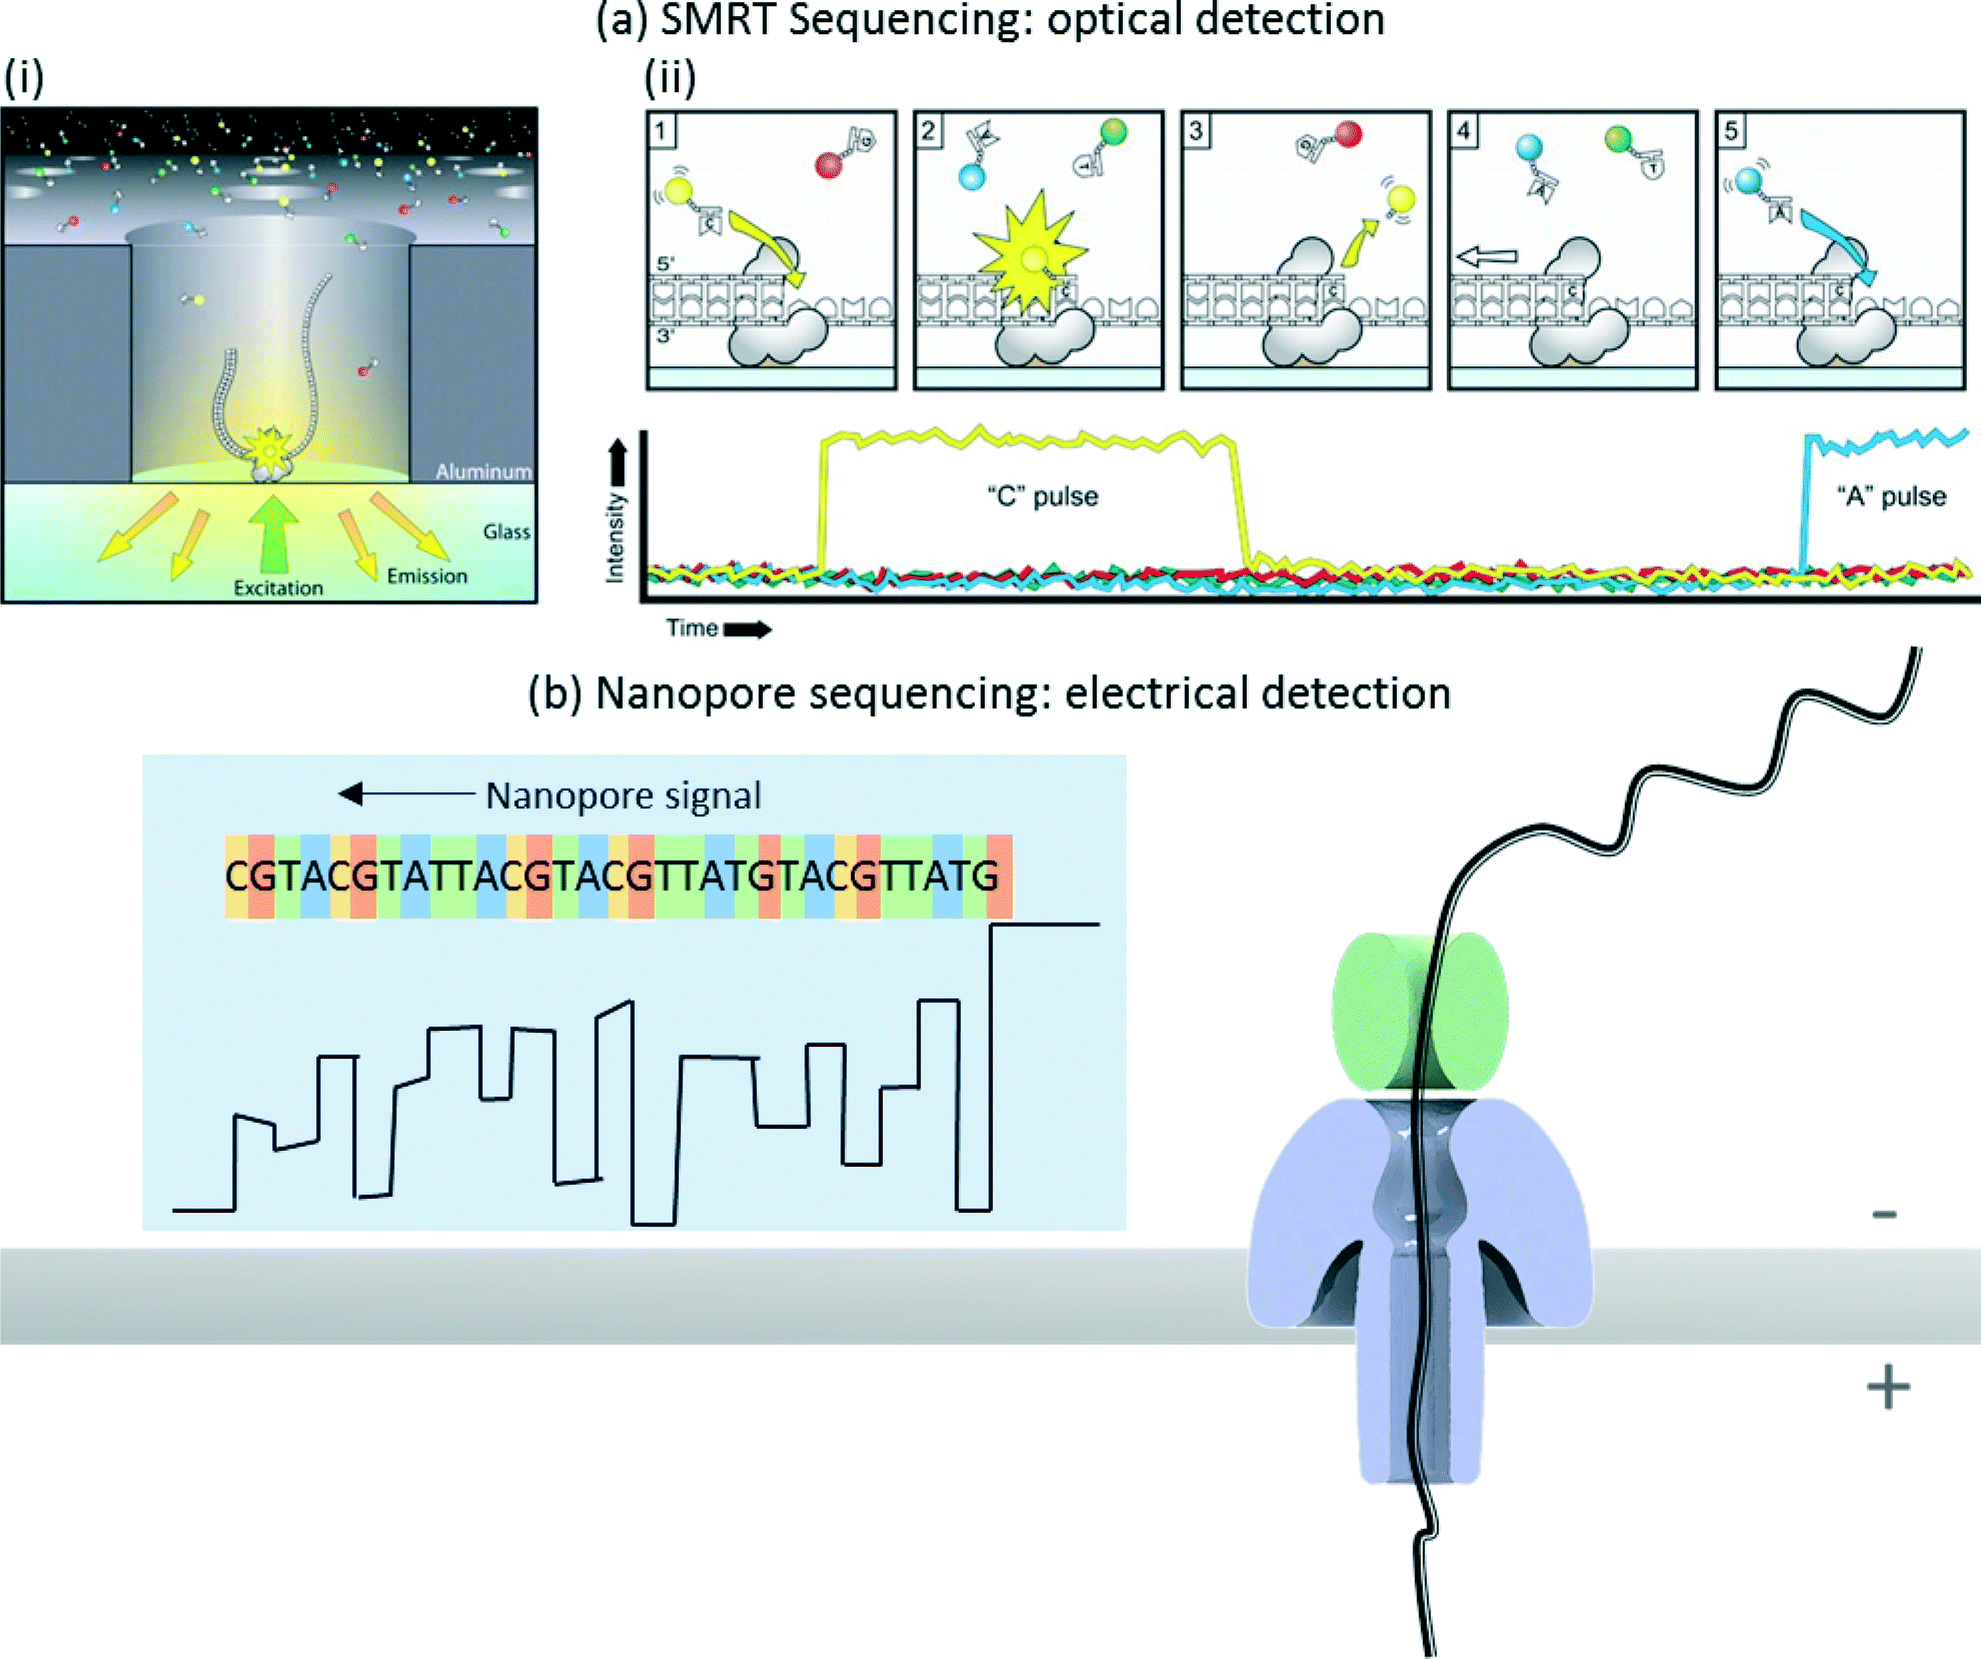
\includegraphics[width=0.8\textwidth]{c2_genomics/sequencing_smrt_nano_03.png}
  \end{figure}
\end{frame}

\subsection{测序技术的比较}
\begin{frame}
  \frametitle{测序 | 比较 | 公司}
  \begin{figure}
    \centering
    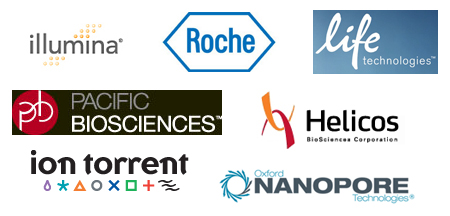
\includegraphics[width=0.9\textwidth]{c2_genomics/sequencing_logo_01.jpg}
  \end{figure}
\end{frame}

\begin{frame}
  \frametitle{测序 | 比较 | 三代}
  \begin{figure}
    \centering
    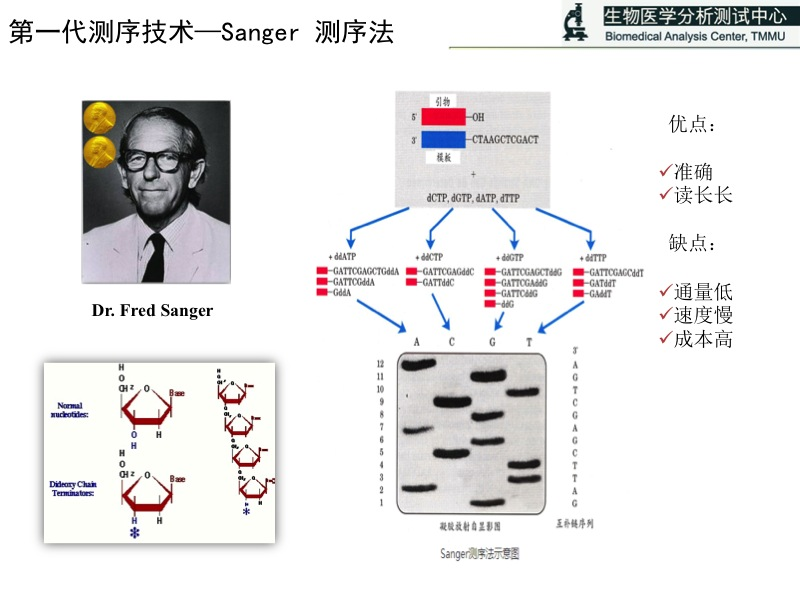
\includegraphics[width=0.9\textwidth]{c2_genomics/sequencing_compare_20.jpg}
  \end{figure}
\end{frame}

\begin{frame}
  \frametitle{测序 | 比较 | 三代}
  \begin{figure}
    \centering
    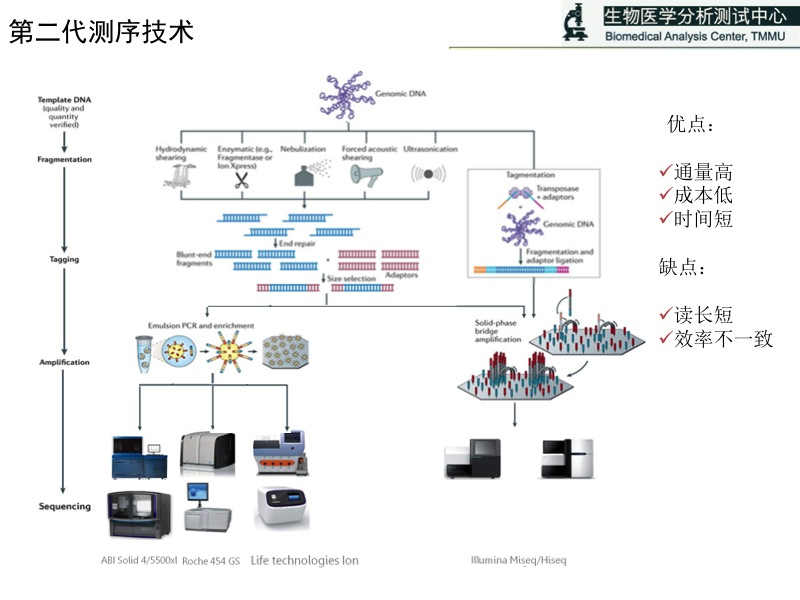
\includegraphics[width=0.9\textwidth]{c2_genomics/sequencing_compare_21.jpg}
  \end{figure}
\end{frame}

\begin{frame}
  \frametitle{测序 | 比较 | 三代}
  \begin{figure}
    \centering
    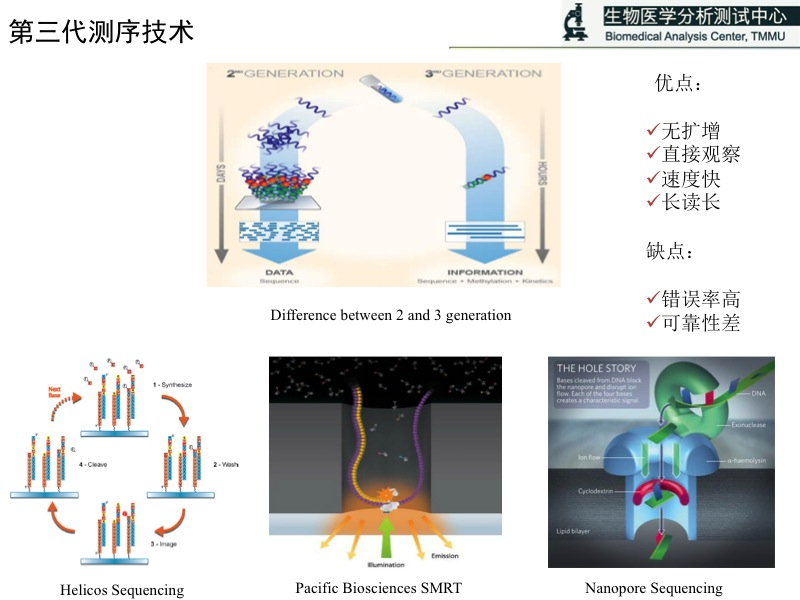
\includegraphics[width=0.85\textwidth]{c2_genomics/sequencing_compare_22.jpg}
  \end{figure}
\end{frame}

\begin{frame}
  \frametitle{测序 | 比较 | 三代}
  \begin{figure}
    \centering
    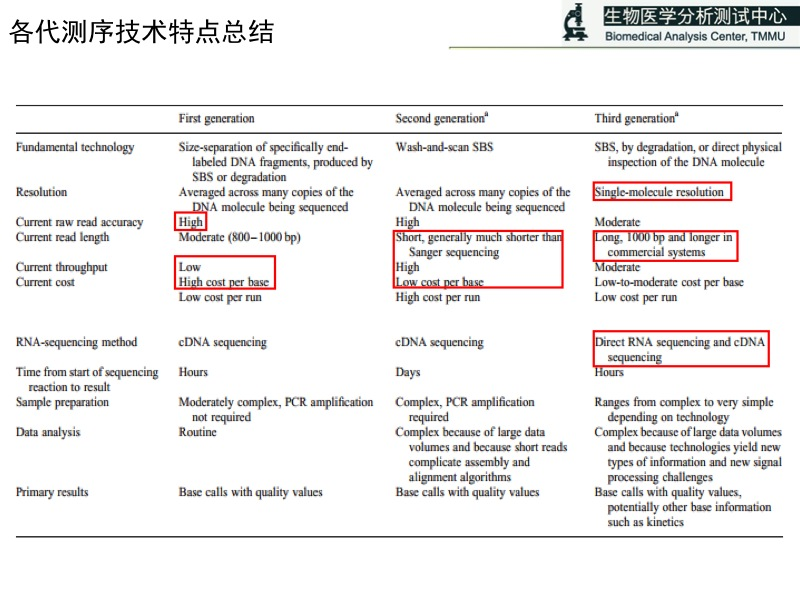
\includegraphics[width=0.9\textwidth]{c2_genomics/sequencing_compare_23.jpg}
  \end{figure}
\end{frame}

\begin{frame}
  \frametitle{测序 | 比较 | 三代}
  \begin{figure}
    \centering
    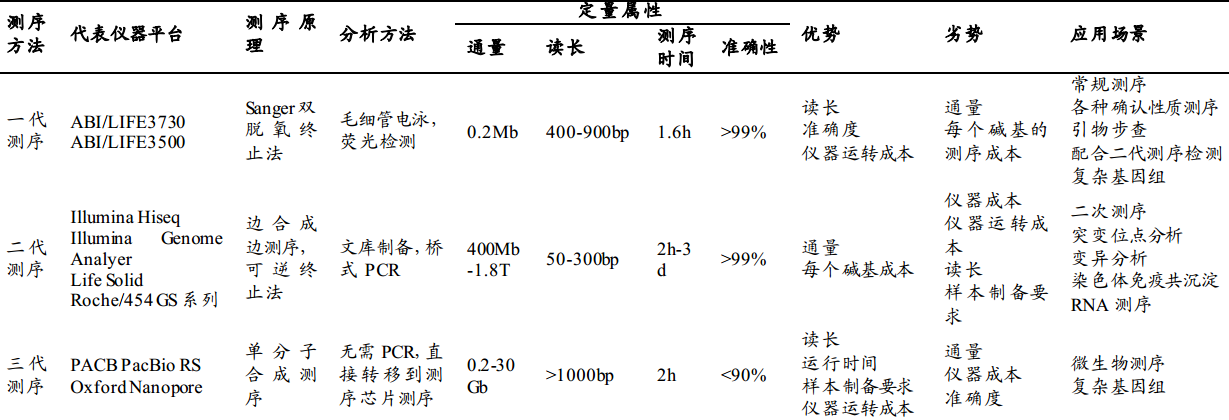
\includegraphics[width=\textwidth]{c2_genomics/sequencing_compare_06.png}
  \end{figure}
\end{frame}

